\documentclass[dvipsnames]{article}
\usepackage[utf8]{inputenc}
\usepackage[left=3cm, right=3cm, top=2cm]{geometry}
\title{Brass}
\author{Silvin Willemsen}
\date{March 2020}

\usepackage{natbib}
\usepackage{graphicx}
\usepackage{appendix}
\usepackage{amsmath}
\usepackage{amsfonts}
\usepackage{amssymb}
\usepackage{cases}
\usepackage[]{algorithm2e, setspace}
\usepackage{tikz}
\usetikzlibrary{decorations.markings}
\usepackage{xcolor}
\def\SBcomment[#1]{\textcolor{red}{#1}}
\def\SWcomment[#1]{\textcolor{blue}{#1}}
\def\SScomment[#1]{\textcolor{green}{#1}}
\def\type[#1]{\textcolor{purple}{#1}}

\def\mystrut{\rule[-.2\baselineskip]{0pt}{\baselineskip}}
\usepackage{mathtools}

\def\dxp{\delta_{x+}}
\def\dxm{\delta_{x-}}
\def\mup{\mu_{x+}}
\def\mum{\mu_{x-}}
\def\Sp{S_{l+1/2}}
\def\Sm{S_{l-1/2}}
\def\Psilp{\Psi_{l+1}^n}
\def\Psilm{\Psi_{l-1}^n}
\def\Psinp{\Psi_l^{n+1}}
\def\Psinm{\Psi_l^{n-1}}
\def\Psiln{\Psi_l^n}
\def\Sbar{\bar S_l}
\def\z{z^{-1}}
\def\muTT{\mu_{tt}}
\def\dtd{\delta_{t\cdot}}
\begin{document}
\maketitle

\section{Introduction}
This document shows the work done and documentation on the brass part of the PhD.

Main references are \cite{Bilbao2009} and \cite{Bilbao2018}.

\section{Variable cross-section}
\subsection{Preamble}
Schemes with variable cross-section behave best (have the greatest band-width) when stretched coordinates are used. Following Section 5.3 of \cite{Bilbao2009}, we can devine a new coordinate $\alpha = \alpha(x)$ where the map $x\rightarrow\alpha$ is ``smooth and one-to-one" (i.e. if $x_1\leq x_2$ then $\alpha_1\leq \alpha_2$). Partial derivatives are as follows:
\begin{equation}
   \partial_x \quad\longrightarrow\quad \alpha'\partial_\alpha \qquad \text{and} \qquad \partial_x^2\quad \longrightarrow\quad\alpha'\partial_\alpha\left(\alpha'\partial_\alpha\right),
\end{equation}
with $\alpha'= \partial \alpha/\partial x$ which describes the rate-of-change of grid spacing with respect to the original grid spacing. In discrete time, a centered approximation for the second spatial derivative is
\begin{equation}\label{eq:secondOrderVarying}
    \delta_{xx} \quad \longrightarrow \quad \alpha'\delta_{\alpha+}\big((\mu_{\alpha-}\alpha')\delta_{\alpha-}\big).
\end{equation}
This operator applied to a grid function $u_l^n$ and expanded yields
\begin{equation}
    \frac{\alpha'_l}{2h^2} \Big((\alpha'_{l+1}+\alpha'_l)u_{l+1}^n + (\alpha'_l+\alpha'_{l-1})u_{l-1}^n - (\alpha'_{l+1}+2\alpha'_l+\alpha'_{l-1})u_l^n\Big),
\end{equation}
or
\begin{equation}
    \frac{\alpha'_l}{h^2}\Big((\mu_{\alpha+}\alpha_l')u_{l+1}^n+(\mu_{\alpha-}\alpha_l')u_{l-1}^n-2(\mu_{\alpha\alpha}\alpha'_l)u_l^n\Big)
\end{equation}
\subsubsection{String of varying cross-section}
The PDE of an ideal string with a varying cross-section is
\begin{equation}\label{eq:idealVarying}
    \epsilon^2\partial_t^2u=c_0^2\partial^2_xu,
\end{equation}
where $c_0^2 = T_0/\rho A_0$ is the reference wave-speed (in m/s) and $\epsilon = \epsilon(x)$ is a spatially varying factor (in ?unit?). Using Eq. \eqref{eq:secondOrderVarying} where $ \alpha'\rightarrow\epsilon$ we can rewrite Eq. \eqref{eq:idealVarying} to
\begin{align}
    \epsilon^2\partial_t^2u&=c_0^2\epsilon\partial_\alpha(\epsilon\partial_\alpha u),\\
    \epsilon\partial_t^2u&=c_0^2\partial_\alpha(\epsilon\partial_\alpha u),
\end{align}

% The obvious finite difference scheme for this would be
% \begin{equation}
%     \epsilon^2(x)\delta_{tt}u=c_0^2\delta_{xx}u.
% \end{equation}
% U
\subsection{Webster's equation}
The first main difference between the 1D brass PDE and the 1D wave equation is the possibility of having a variable cross-section. Following Section 19.3 from \cite{Bilbao2018}, the PDE for a 1D (axially symmetric) acoustic tube with variable cross-section is (also known as \textit{Webster}'s equation)
\begin{equation}\label{eq:webstersPDE}
    S\partial_t^2\Psi = c^2\partial_x(S\partial_x\Psi),
\end{equation}
with \textit{acoustic potential} $\Psi = \Psi(x,t)$ (m$^2$/s), $S = S(x)$ is the cross sectional area (m$^2$) and wave speed $c$ (m/s).

\subsection{Discretisation}
Introducing interleaved gridpoints at $n-1/2$ and $n+1/2$ for $S$, a we can discretise Eq. \eqref{eq:webstersPDE} (following \cite{Bilbao2018}) to
\begin{equation}\label{eq:discWebster}
    \Sbar \delta_{tt}\Psi^n_l = c^2\dxp(\Sm(\delta_{x-}\Psiln)),
\end{equation}
where
\begin{equation}
    \Sbar = \mu_{t+}\Sm = \frac{\Sp + \Sm}{2}.
\end{equation}
The right side of the equation in \eqref{eq:discWebster} contains an operator applied to two grid functions ($S$ and $\Psi$) multiplied onto each other. In order to expand this, we need to use the product rule (Eq. (2.23) in \cite{Bilbao2009}) which is
\begin{equation}
    \dxp (u_lw_l) = (\dxp u_l)(\mup{w_l}) + (\mup u_l)(\dxp w_l).
\end{equation}
In the case of \eqref{eq:discWebster}, $u_l \triangleq \Sm$ and $w_l \triangleq \dxm\Psiln$. Expanding (retaining the notation for $\Sbar$) and solving for $\Psinp$ yields (Appendix \ref{app:webstersUpdateEq})
\begin{equation}
    \Psinp = 2(1-\lambda^2)\Psiln-\Psinm+ \frac{\lambda^2\Sp}{\Sbar}\Psilp + \frac{\lambda^2\Sm}{\Sbar}\Psilm,\label{eq:webstersUpdateEq}
\end{equation}
which is identical to Eq. (19.51) in \cite{Bilbao2018}.

\subsection{Boundary Conditions}
The choices for boundary conditions in an acoustic tube are open and closed, defined as \cite{Bilbao2018}
\begin{equation}
    \begin{split}
        \partial_t\Psi &= 0\ \text{(open, Dirichlet)}\\
        \partial_x\Psi &= 0\ \text{(closed, Neumann)},
    \end{split}
\end{equation} 
at the ends of the tube. This might be slightly counter-intuitive as in the case of a string ``closed" might imply the ``clamped" or Dirichlet boundary condition. The opposite can be intuitively shown imagining a wave front with a positive acoustic potential moving through a tube and hitting a closed end. What comes back is also a wave front with a positive acoustic potential, i.e., the sign of the potential does not flip, which also happens using the free or Neumann condition for the string.

In this case we follow \cite[Chapter 9]{Bilbao2009} and use the following
\begin{equation}\label{eq:openClosed}
    \partial_x\Psi(0, t) = 0 \quad \text{and} \quad \partial_t\Psi(L, t) = 0
\end{equation}
i.e. closed at the left end and open at the right end. In discrete time we have two choices for the closed condition
\begin{equation}\label{eq:centNonCentBound}
\begin{split}
    \delta_{x\cdot}\Psi_0^n &= 0 \ \Rightarrow \ \Psi_{-1}^n = \Psi_1^n \quad \text{(centered)}\\
    \delta_{x-}\Psi_0^n &= 0\  \Rightarrow \ \Psi_{-1}^n = \Psi_0^n\quad \text{(non-centered)}
\end{split}
\end{equation}
At the left boundary we can now solve Eq. \eqref{eq:webstersUpdateEq} for the centered case:
\begin{equation}
    \begin{aligned}
        \Psi_0^{n+1} &= 2(1-\lambda^2)\Psi_0^n-\Psi_0^{n-1}+ \frac{\lambda^2S_{1/2}}{\bar S_0}\Psi_1^n + \frac{\lambda^2S_{-1/2}}{\bar S_0}\Psi_{-1}^n\nonumber\\
        \Psi_0^{n+1} &= 2(1-\lambda^2)\Psi_0^n-\Psi_0^{n-1}+ \frac{\lambda^2(S_{1/2}+S_{-1/2})}{\bar S_0}\Psi_1^n\nonumber\\
         \Psi_0^{n+1} &= 2(1-\lambda^2)\Psi_0^n-\Psi_0^{n-1}+ 2\lambda^2\Psi_1^n,
    \end{aligned}
\end{equation}
and the non-centered case
\begin{equation}\label{eq:nonCentLeft}
    \Psi_0^{n+1} = 2(1-\lambda^2)\Psi_0^n-\Psi_0^{n-1}+ \frac{\lambda^2S_{1/2}}{\bar S_0}\Psi_1^n + \frac{\lambda^2S_{-1/2}}{\bar S_0}\Psi_0^n.
\end{equation}
As can be seen from the equations above, we need undefined points $\bar S_0$ and $S_{-1/2}$. At the left boundary, we set $\bar S_0 = S_0$ from which, we can calculate $S_{-1/2}$:
\begin{equation}
        S_0 = \frac{1}{2}(S_{1/2} + S_{-1/2}) \ \Rightarrow \  S_{-1/2}
        = 2S_0 - S_{1/2}
\end{equation}
The same can be done for the right boundary ($\bar S_N = S_N$) if this is chosen to be anything else but open (e.g., closed or radiating -- see Section \ref{sec:radiating}):
\begin{equation}
    S_N = \frac{1}{2}(S_{N+1/2} + S_{N-1/2}) \ \Rightarrow \ S_{N+1/2} = 2S_N - S_{N-1/2}.
\end{equation}
For now though, we follow the conditions given in \eqref{eq:openClosed} and we can simply set the right boundary to its initial state
\begin{equation}
    \Psi_N^n = \Psi_N^0
\end{equation}
which is normally $0$. A more realistic open end is a radiating one, which can be found below.
\subsubsection{Radiating end}\label{sec:radiating}
We can change the condition presented in Eq. \eqref{eq:openClosed} to a radiating end,
\begin{equation}\label{eq:radCont}
    \partial_x\Psi(L,t) = -a_1\partial_t\Psi(L,t)-a_2\Psi(L,t)
\end{equation}
where \cite{Bilbao2009}
\begin{equation}
    a_1 = \frac{1}{2(0.8216)^2c} \quad \text{and} \quad a_2 = \frac{L}{0.8216\sqrt{S_0S(1)/\pi}}.
\end{equation}
taken from \cite{Atig2004} and are valid for a tube terminating on an infinite plane. The terms in Eq. \eqref{eq:radCont} are a damping and an inertia term where $a_1$ is a loss coefficient and $a_2$ is the \textbf{inertia coefficient}. The centered and non-centered case are defined as
\begin{equation}\label{eq:rightBoundaryConditions}
\begin{split}
    \delta_{x\cdot}\Psi_N^n &= 0 \ \Rightarrow \ \Psi_{N+1}^n = \Psi_{N-1}^n \quad \text{(centered)}\\
    \delta_{x+}\Psi_N^n &= 0\  \Rightarrow \ \Psi_{N+1}^n = \Psi_N^n\qquad \text{(non-centered)}
\end{split}
\end{equation}
First, we solve Eq. \eqref{eq:radCont} for the centered (Eq. (9.16) in \cite{Bilbao2009})
\begin{equation}\label{eq:centRadBound}
    \delta_{x\cdot}\Psi_N^n = -a_1\dtd\Psi_N^n - a_2\mu_{t\cdot}\Psi_N^n
\end{equation}
which can be expanded and solved for $\Psi_{N+1}^n$ according to
\begin{align}
    \frac{1}{2h}(\Psi_{N+1}^n - \Psi_{N-1}^n) &= -\frac{a_1}{2k}(\Psi_N^{n+1} - \Psi_N^{n-1}) - \frac{a_2}{2}(\Psi_N^{n+1} + \Psi_N^{n-1})\nonumber\\
    \Psi_{N+1}^n &= h\left(-\frac{a_1}{k}(\Psi_N^{n+1} - \Psi_N^{n-1}) - a_2(\Psi_N^{n+1} + \Psi_N^{n-1})\right) + \Psi_{N-1}^n,
\end{align}
which can be substituted into Eq. \eqref{eq:webstersUpdateEq} (Appendix \ref{app:centeredRad}) 
\begin{equation}
    \Psi_N^{n+1} = \frac{2(1-\lambda^2)\Psi_N^n-\Psi_N^{n-1}+\frac{h\lambda^2S_{N+1/2}}{\bar S_N}\left(\frac{a_1}{k}-a_2\right)\Psi_N^{n-1} + 2\lambda^2\Psi_{N-1}^n}{\left(1+\left(\frac{a_1}{k}+a_2\right)\frac{h\lambda^2S_{N+1/2}}{\bar S_N}\right)}.
\end{equation}
The same can be done for the non-centered case (Eq. (9.15) in \cite{Bilbao2009})
\begin{equation}\label{eq:nonCentRadBound}
    \delta_{x+}\Psi_N^n = -a_1\dtd\Psi_N^n - a_2\mu_{t\cdot}\Psi_N^n
\end{equation}
which when solved for $\Psi_{N+1}^n$ yields
\begin{align}
    \frac{1}{h}(\Psi_{N+1}^n - \Psi_{N}^n) &= -\frac{a_1}{2k}(\Psi_N^{n+1} - \Psi_N^{n-1}) - \frac{a_2}{2}(\Psi_N^{n+1} + \Psi_N^{n-1})\nonumber\\
        \Psi_{N+1}^n &= h\left(-\frac{a_1}{2k}(\Psi_N^{n+1} - \Psi_N^{n-1}) - \frac{a_2}{2}(\Psi_N^{n+1} + \Psi_N^{n-1})\right) + \Psi_{N}^n.
\end{align}
Substituted into Eq. \eqref{eq:webstersUpdateEq} yields (Appendix \ref{app:nonCentRad})
\begin{equation}
    \Psi_N^{n+1} = \frac{2(1-\lambda^2)\Psi_N^n-\Psi_N^{n-1}+\frac{h\lambda^2S_{N+1/2}}{\bar S_N}\left(\frac{a_1}{2k}-\frac{a_2}{2}\right)\Psi_N^{n-1} + \frac{\lambda^2S_{N+1/2}}{\bar S_N}\Psi_{N}^n + \frac{\lambda^2S_{N-1/2}}{\bar S_N}\Psi_{N-1}^n}{\left(1+\left(\frac{a_1}{2k}+\frac{a_2}{2}\right)\frac{h\lambda^2S_{N+1/2}}{\bar S_N}\right)}.
\end{equation}

\subsection{Energy}
In continuous time, the rate of change of the energy of a PDE can be obtained by taking the inner product with the first-order time derivative of the state \SWcomment[Say something here about obtaining units of power ``in this case, this means to multiply with the first time-derivative of the state $\Psi$]. Using state $\Psi$, this yields
\begin{equation}
    \frac{d\mathfrak{H}}{dt} = \langle \partial_t\Psi, \text{PDE} \rangle\quad \text{where} \quad \mathfrak{H} = \mathfrak{T} + \mathfrak{D},
\end{equation}
with total energy (or Hamiltonian) $\mathfrak{H}$, kinetic energy $\mathfrak{T}$ and potential energy $\mathfrak{D}$.

In discrete time, the energy of a FDS can be obtained by taking the inner product the equation with $\dtd\Psiln$ according to 
\begin{equation}\label{eq:energyForm}
    \delta_{t+}\mathfrak{h} = \langle \dtd\Psiln,\text{FDS}\rangle \quad \text{where} \quad \mathfrak{h} = \mathfrak{t} + \mathfrak{v},
\end{equation}
where $\mathfrak{h}$, $\mathfrak{t}$ and $\mathfrak{v}$ are the discrete counterparts of $\mathfrak{H}$, $\mathfrak{T}$ and $\mathfrak{D}$.

With a boundary term present, Eq. \eqref{eq:energyForm} becomes
\begin{equation}\label{eq:energyFormBoundary}
    \delta_{t+}\mathfrak{h} = \mathfrak{b}.
\end{equation}
In the case of the radiating boundary -- with an inertia and damping term -- the energy equation is of the form
\begin{equation}\label{eq:radiatingEnergyForm}
    \delta_{t+}(\mathfrak{h}+\mathfrak{h}_\text{b}) = -\mathfrak{q}_\text{b},
\end{equation}
where $\mathfrak{h}_\text{b}$ is the energy stored by the boundary and $\mathfrak{q}_\text{b}$ is the loss energy.
\subsubsection{Kinetic Energy}
The (discrete) kinetic energy of the system $\mathfrak{t}$ of Webster's equation in Eq. \eqref{eq:discWebster} is found by taking the inner product of the left side of the equation with $\dtd\Psi$ according to
\begin{equation}
    \delta_{t+}\mathfrak{t} = \langle\dtd\Psiln,\Sbar \delta_{tt}\Psiln  \rangle_\mathcal{D},
\end{equation}
where domain $\mathcal{D}\in [0, N]$. As $\Sbar$ is merely a coefficient here, we can use identity (2.22a) from \cite{Bilbao2009} and rewrite to
\begin{equation}
    \begin{aligned}
    \delta_{t+}\left(\frac{1}{2}\sum_\mathcal{D}h\Sbar(\delta_{t-}\Psiln)^2\right)\quad \Rightarrow \quad \delta_{t+}\left(\frac{1}{2}\sum_\mathcal{D}h(\sqrt{\Sbar}\delta_{t-}\Psiln)^2\right)
    \end{aligned}.
\end{equation}
We place $\Sbar$ as a square-root in the equation, so that we can rewrite it as a norm over a domain as
\begin{equation}
    \mathfrak{t} = \frac{1}{2}\lVert\sqrt{\bar S_l}\delta_{t-}\Psiln\rVert_\mathcal{D}^2
\end{equation}
just like Eq. (9.14) in \cite{Bilbao2009}. When the boundaries of the scheme are centered we need to use a primed inner product (Eq. (5.23) in \cite{Bilbao2009}) as Bilbao explains right below Eq. (5.28) in \cite{Bilbao2009}:
\begin{equation}\label{eq:primedInnerProduct}
    \langle f,g \rangle_{\mathcal{D}}'= \sum_{l = 1}^{N-1}hf_lg_l + \frac{h}{2}f_0g_0 + \frac{h}{2}f_Ng_N,
\end{equation} 
However, in the spatially varying case (which we are dealing with here), a more general weighted inner product needs to be used, which for a domain $\mathcal{D} = [0,\hdots,N]$ is defined as (as given in Eq. (5.38) in \cite{Bilbao2009}) 
\begin{equation}\label{eq:weightedInnerProduct}
    \langle f,g \rangle_{\mathcal{D}}^{\epsilon_\text{l}, \epsilon_\text{r}}= \sum_{l = 1}^{N-1}hf_lg_l + \frac{\epsilon_\text{l}}{2}hf_0g_0 + \frac{\epsilon_\text{r}}{2}hf_Ng_N,
\end{equation}
where free parameters $\epsilon_\text{l}, \epsilon_\text{r} > 0$ `tune' the weighting of the boundaries. If $\epsilon_\text{l} = \epsilon_\text{r} = 1$, Eq. \eqref{eq:weightedInnerProduct} reduces to the primed inner product from Eq. \eqref{eq:primedInnerProduct}. For the kinetic energy, we now have
\begin{equation}
    \mathfrak{t} = \frac{1}{2}\left(\lVert\sqrt{\bar S_l}\delta_{t-}\Psiln \rVert_\mathcal{D}^{\epsilon_\text{l}, \epsilon_\text{r}}\right)^2,
\end{equation}
which, when expanded, yields
\begin{align}
    \mathfrak{t} &= \frac{1}{2}\left(\sqrt{\sum_{l=1}^{N-1}h\left(\sqrt{\bar S_l}\delta_{t-}\Psiln\right)^2 + \frac{\epsilon_\text{l}}{2}h\left(\sqrt{\bar S_0 }\delta_{t-}\Psi_0^n\right)^2 + \frac{\epsilon_\text{r}}{2}h\left(\sqrt{\bar S_N }\delta_{t-}\Psi_N^n\right)^2}\right)^2\nonumber\\
     &=\frac{1}{2}\left(\sum_{l=1}^{N-1}h\bar S_l(\delta_{t-}\Psiln)^2 + \frac{\epsilon_\text{l}}{2}h\bar S_0 (\delta_{t-}\Psi_0^n)^2 + \frac{\epsilon_\text{r}}{2}h\bar S_N (\delta_{t-}\Psi_N^n)^2\right)    .
\end{align}
The values of $\epsilon_\text{l}$ and $\epsilon_\text{r}$ can be calculated by performing the same energy analysis techniques on the right side of the equation to obtain the potential energy and the boundary terms, and will be given below.


\subsubsection{Potential Energy}
It can be shown that \eqref{eq:discWebster} is equal to
\begin{equation}
    \Sbar \delta_{tt}\Psi^n_l = c^2\dxm\big(\Sp(\dxp\Psiln)\big),
\end{equation}
i.e. changing the signs of the operators at the left side of the equation. Using $(\mup S = S_{l+1/2})$, we define for the non-centered case
\begin{equation}\label{eq:potContEnergy}
c^2\langle \dtd\Psiln, \dxm((\mup S)(\dxp\Psiln))\rangle_\mathcal{D},
\end{equation}
which, using summation by parts (see Appendix \ref{app:summation}) can be written as (see Appendix \ref{app:potDerivNonCent})
\begin{equation}\label{eq:discROCPotBoundNonCent}
\underbrace{-c^2\langle(\mu_{x+}S)\dtd\dxp\Psiln, \dxp\Psiln\rangle_{\underline{\mathcal{D}}}}_{\let\scriptstyle\textstyle\delta_{t+}\mathfrak{v}} + \underbrace{c^2\Big( (\dtd\Psi_N^n)(\mup S_N)(\dxp\Psi_N^n) -(\dtd\Psi_0^n)(\mum S_0)(\dxm \Psi_0^n)\Big)}_{\mathfrak{b}},
\end{equation}
with boundary energy term $\mathfrak{b}$ as seen in Eq. \eqref{eq:energyFormBoundary} (for more detail, see Section \ref{sec:boundaries}).
Notice that $\mup S$ has been moved to the other side of the inner product according to match Eq. (9.14) in \cite{Bilbao2009}. We can also take $\mup S$ out of the inner product (as it is a coefficient here)
\begin{equation}
    -c^2(\mu_{x+}S)\langle\dtd\dxp\Psiln, \dxp\Psiln\rangle_{\underline{\mathcal{D}}},
\end{equation}
to use Eq. (2.22b) to end up with 
\begin{equation}
    \delta_{t+}\mathfrak{v} = \delta_{t+}\left(-\frac{c^2}{2}(\mu_{x+}S)\langle\dxp\Psiln, e_{t-}\dxp\Psiln\rangle_{\underline{\mathcal{D}}}\right),
\end{equation}
where (again, as $S$ acts as a coefficient) $\mup S$ can be inserted back into the inner product
\begin{equation}
   \mathfrak{v}=-\frac{c^2}{2}\langle(\mu_{x+}S)\dxp\Psiln, e_{t-}\dxp\Psiln\rangle_{\underline{\mathcal{D}}}.
\end{equation}
See Appendix \ref{app:proof} for a proof of this.

For the centered case, we need to use the weighted inner product as defined in \eqref{eq:weightedInnerProduct}:
\begin{equation}\label{eq:potContEnergyCent}
c^2\langle \dtd\Psiln, \dxm((\mup S)(\dxp\Psiln))\rangle_\mathcal{D}^{\epsilon_\text{l},\epsilon_\text{r}},
\end{equation}
which, after summation by parts becomes (see Appendix \ref{app:potDerivCent}) (\textit{Note that $\mathfrak{b}_\text{l}$ is subtracted})
\begin{equation}\label{eq:discROCPotBoundCent}
    \underbrace{-c^2\langle(\mu_{x+}S)\dtd\dxp\Psiln, \dxp\Psiln\rangle_{\underline{\mathcal{D}}}}_{\let\scriptstyle\textstyle\delta_{t+}\mathfrak{v}}\ +\ \mathfrak{b}_\text{r} - \mathfrak{b}_\text{l},
\end{equation}
where
\begin{subequations}
\begin{align}
 \mathfrak{b}_\text{r} &= c^2(\dtd\Psi_N^n)\left(\frac{\epsilon_\text{r}}{2}S_{N+1/2}(\dxp \Psi_N^n) + \left(1-\frac{\epsilon_\text{r}}{2}\right)S_{N-1/2}(\dxm\Psi_N^n)\right), \\
 \mathfrak{b}_\text{l} &= c^2(\dtd\Psi_0^n)\left(\frac{\epsilon_\text{l}}{2}S_{-1/2}(\dxm\Psi_0^n)+\left(1-\frac{\epsilon_\text{l}}{2}\right)S_{1/2}(\dxp \Psi_0^n))\right).
\end{align}
\end{subequations}
For the special cases of $\epsilon_\text{r} = S_{N-1/2}/\mu_{xx}S_N$ and $\epsilon_\text{l} = S_{1/2}/\mu_{xx}S_0$ the boundary terms become strictly dissipative (see Appendix \ref{app:potDerivCent} for the (painstaking) derivation of this)
\begin{subequations}\label{eq:centStrictDissip}
\begin{align}
    \mathfrak{b}_\text{r} &= c^2 (\dtd\Psi_N^n)S_{N-1/2}(2-\epsilon_\text{r})(\delta_{x\cdot}\Psi_N^n)\label{eq:centStrictDissipRight}\\
    \mathfrak{b}_\text{l} &= c^2 (\dtd\Psi_0^n)S_{1/2}(2-\epsilon_\text{l})(\delta_{x\cdot}\Psi_0^n)\label{eq:centStrictDissipLeft}
\end{align}
\end{subequations}

\subsubsection{Boundaries}\label{sec:boundaries}
Recalling the boundary term from Eq. \eqref{eq:discROCPotBoundNonCent} 
\begin{equation}
    \mathfrak{b} = \underbrace{ c^2(\dtd\Psi_N^n)(\mup S_N)(\dxp\Psi_N^n)}_{\mathfrak{b_\text{r}} \text{ (right boundary)}} -\underbrace{c^2(\dtd\Psi_0^n)(\mum S_0)(\dxm \Psi_0^n)}_{\mathfrak{b}_\text{l} \text{ (left boundary)}}
\end{equation}
We first consider the left boundary. Recalling Eq. \eqref{eq:centNonCentBound}, we see that for the non-centered case, $\Psi_{-1}^n = \Psi_0^n$. This means that $(\dxm\Psi_0^n) = 0 $ yielding
\begin{equation}
    \mathfrak{b}_\text{l} = c^2(\dtd\Psi_0^n)(S_{-1/2})(0) = 0.
\end{equation}
For the centered case, $\Psi_{-1}^n = \Psi_1^n$. Substituting this into the equation for the left boundary yields
\begin{equation}
    \mathfrak{b}_\text{l} = \frac{c^2}{2kh}(\Psi_0^{n+1} - \Psi_0^{n-1})(S_{-1/2})(\Psi_0^n - \Psi_1^n)
\end{equation}
Continuing with the right boundary it can be seen that the lossless case, where $(\dtd \Psi_N^n) = 0$ results in 
\begin{equation}
    \mathfrak{b}_\text{r} = c^2(0)(S_{N+1/2})(\dxp\Psi_N^n) = 0.
\end{equation}
The damped condition, however, is much more interesting. In the non-centered case, we can substitute this into the definition found in Eq. \eqref{eq:nonCentRadBound} to get
\begin{equation}
    \mathfrak{b}_\text{r} = c^2(\dtd\Psi_N^n)( S_{N+1/2})(-a_1\dtd\Psi_N^n - a_2\mu_{t\cdot}\Psi_N^n),
    \end{equation}
    and using the identity
    \begin{equation}
    (\dtd u)(\mu_{t\cdot}u) = \frac{1}{2} \dtd(u)^2,
\end{equation}
we end up with
\begin{equation}
    \mathfrak{b}_\text{r} = c^2 S_{N+1/2}\left(-a_1(\dtd\Psi_N^n)^2 - \frac{a_2}{2}\dtd(\Psi_N^n)^2\right).
\end{equation}
As this boundary both has damping with energy term $\mathfrak{q}_\text{b}$ and inertia with stored energy $\mathfrak{h}_\text{b}$ it can be written in the form found in Eq. \eqref{eq:radiatingEnergyForm}. First, substituting $\mathfrak{b}_\text{r}$ into Eq. \eqref{eq:energyFormBoundary} yields %we can subdivide $\mathfrak{b}_r$ as follows:
\begin{align}
\delta_{t+}\mathfrak{h} &= c^2 S_{N+1/2}\left(-a_1(\dtd\Psi_N^n)^2 - \frac{a_2}{2}\dtd(\Psi_N^n)^2\right)\\
\delta_{t+}\mathfrak{h} + \frac{c^2S_{N+1/2}a_2}{2}\delta_{t+}\mu_{t-} (\Psi_N^n)^2 &= -c^2S_{N+1/2}a_1(\dtd\Psi_N^n)^2
\end{align}
%
\begin{equation}
    \begin{gathered}
    \delta_{t+}\left(\mathfrak{h} + \mathfrak{h}_\text{b}\right) = -\mathfrak{q}_\text{b} \quad \text{where}\\
    \mathfrak{h}_\text{b} = \frac{c^2S_{N+1/2}a_2}{2}\mu_{t-} (\Psi_N^n)^2 \quad \text{and} \quad
    \mathfrak{q}_\text{b} = c^2S_{N+1/2}a_1(\dtd\Psi_N^n)^2,
    \end{gathered}
\end{equation}

which is exactly what we find in \cite{Bilbao2009} underneath Eq. (9.15).

For the centered case, recalling Eqs. \eqref{eq:centRadBound} and \eqref{eq:centStrictDissipRight} we can follow similar steps to end up at
\begin{equation}
    \mathfrak{b}_\text{r} = c^2S_{N-1/2}(2-\epsilon_\text{r})(-a_1(\dtd\Psi_N^n)^2-\frac{a_2}{2}\dtd(\Psi_N^n)^2).
\end{equation}
When written in the form found in Eq. \eqref{eq:radiatingEnergyForm} we obtain
\begin{equation}
    \begin{gathered}
    \delta_{t+}\left(\mathfrak{h} + \mathfrak{h}_\text{b}\right) = -\mathfrak{q}_\text{b} \quad \text{where}\\
    \mathfrak{h}_\text{b} = \frac{c^2S_{N-1/2}(2-\epsilon_\text{r})a_2}{2}\mu_{t-} (\Psi_N^n)^2 \quad \text{and} \quad
    \mathfrak{q}_\text{b} = c^2S_{N-1/2}(2-\epsilon_\text{r})a_1(\dtd\Psi_N^n)^2,
    \end{gathered}
\end{equation}
% The centered case found in Eq. \eqref{eq:centRadBound} needs to be rewritten in the form $\dxp\Psi_N^n = \hdots$ to be able to be substituted into the right boundary term. This is done as follows
% \begin{align}
%     \delta_{x\cdot}\Psi_N^n &= -a_1\dtd\Psi_N^n - a_2\mu_{t\cdot}\Psi_N^n\nonumber\\
%     \Psi_{N+1}^n-\Psi_{N-1}^n &= 2h\left(-a_1\dtd\Psi_N^n - a_2\mu_{t\cdot}\Psi_N^n\right)\nonumber\\
%     \Psi_{N+1}^n-\Psi_N^n+\Psi_N^n-\Psi_{N-1}^n &= 2h\left(-a_1\dtd\Psi_N^n - a_2\mu_{t\cdot}\Psi_N^n\right)\nonumber\\
%     \dxp\Psi_N^n+\dxm\Psi_N^n &= 2\left(-a_1\dtd\Psi_N^n - a_2\mu_{t\cdot}\Psi_N^n\right)\nonumber\\
%     \dxp\Psi_N^n &= 2\left(-a_1\dtd\Psi_N^n - a_2\mu_{t\cdot}\Psi_N^n\right)-\dxm\Psi_N^n
% \end{align}
% which can then be substituted into the right boundary term
% \begin{align}
%     \mathfrak{b}_\text{r} &=  c^2(\dtd\Psi_N^n)(S_{N+1/2})(2\left(-a_1\dtd\Psi_N^n - a_2\mu_{t\cdot}\Psi_N^n\right)-\dxm\Psi_N^n)\nonumber\\
% &= c^2S_{N+1/2}\left(-2a_1(\dtd\Psi_N^n)^2 - a_2\dtd(\Psi_N^n)^2-(\dtd\Psi_N^n)(\dxm\Psi_N^n)\right)
% \end{align}
% \SWcomment[Here, we can write it in the same form as Eq. \eqref{eq:radiatingEnergyForm} with
% \begin{equation}
%     \mathfrak{h}_\text{b} = c^2S_{N+1/2}a_2\mu_{t-} (\Psi_N^n)^2  \quad \text{and} \quad
% \mathfrak{q}_\text{b} = 2c^2S_{N+1/2}a_1(\dtd\Psi_N^n)^2,
% \end{equation}
% with a \textbf{leftover term}
% \begin{equation}
%     \mathfrak{?}_\text{b} = -(\dtd\Psi_N^n)(\dxm\Psi_N^n).
% \end{equation}]
\section{First-order systems}
Until now we have looked at the second-order PDE shown in Eq. \eqref{eq:webstersPDE}. However, according to \cite{Harrison2018}, (apart from being useful for a ``simpler discussion'' of boundary conditions) a system of first-order PDEs equivalent to Webster's equation was shown to be more accurate \cite{Torin2015}. Furthermore, the state of the art \cite{Harrison2018, Harrison2016} works with these schemes and allow to more easily add viscothermal losses.

The system is defined as follows:
\begin{subequations}\label{eq:firstOrderSystem}
\begin{align}
    \frac{S}{\rho_0 c^2}\partial_t p &= -\partial_x(Sv)\label{eq:contPressure}\\
    \rho_0\partial_tv &= -\partial_xp\label{eq:discVelocity}
\end{align}
\end{subequations}
where pressure $p = p(x,t) = \rho_0\partial_t \Psi$ (N/m$^2$) and particle velocity $v = v(x,t) = -\partial_x\Psi$ (m/s) with air density $\rho_0$. Indeed it can be shown by substituting these definitions into Eq. \eqref{eq:contPressure}, Webster's equation is obtained again:
\begin{equation}
  \nonumber
        \frac{S}{\rho_0 c^2}\partial_t(\rho_0 \partial_t\psi) = -\partial_x(S(-\partial_x\Psi))\quad \Longrightarrow \quad S\partial_t^2\psi = c^2\partial_x(S\partial_x\Psi).
\end{equation}
\subsection{Discretisation}
As done in \cite{Harrison2018}, it is useful to place either $p$ or $v$ on an interleaved grid; both in space and time. Following Harrison, we place $v$ on this interleaved grid. Accordingly, system \eqref{eq:firstOrderSystem} is discretised as
\begin{subequations}
    \begin{align}
        \frac{\bar S_l}{\rho_0 c^2}\delta_{t+}p_l^n &= -\delta_{x-}(S_{l+1/2}v_{l+1/2}^{n+1/2}),\label{eq:discPressure}\\
        \rho_0 \delta_{t-}v_{l+1/2}^{n+1/2}&=-\delta_{x+}p_l^n,\label{eq:discVelocity}
    \end{align}
\end{subequations}
after which the update schemes become
\begin{subequations}
    \begin{align}
        p_l^{n+1} &= p_l^n - \frac{\rho_0 c \lambda}{\bar{S}_l}(S_{l+1/2}v_{l+1/2}^{n+1/2}-S_{l-1/2}v_{l-1/2}^{n-1/2}),\label{eq:pressureUpdate}\\
        v_{l+1/2}^{n+1/2} &= v_{l+1/2}^{n-1/2}-\frac{\lambda}{\rho_0 c}(p_{l+1}^n - p_l^n),\label{eq:velocityUpdate}
    \end{align}
\end{subequations}
where (again) $\lambda = ck/h$.

\subsection{Boundary Conditions}\label{sec:boundariesFirstOrder}
In the first-order PDE case, the boundary conditions are defined as follows
\begin{align*}
    p_0^n &= 0, & p_N^n &= 0, & &\text{(Dirichlet),}\\
    \mu_{x-}(S_{1/2}v_{1/2}^n) &= 0, & \mu_{x+}(S_{N-1/2}v_{N-1/2}^n) &= 0, & &\text{(Neumann)},
\end{align*}
for all $n$.

\subsection{Energy}
For the energy analysis of the first-order system presented above, \cite{Harrison2018} is followed. Instead of taking an inner product with $\delta_{t\cdot}\Psi$ we take an inner product with $\mu_{t+}p$ instead. Using the primed inner product from Eq. \eqref{eq:primedInnerProduct}\footnote{We can use the primed rather than the weighted inner product here as the boundary conditions are defined as found in Section \ref{sec:boundariesFirstOrder}.} for Eq. \eqref{eq:discPressure} and after taking all terms to the left-hand side, this yields
\begin{equation}\label{eq:firstOrderPrimed}
    \delta_{t+}\mathfrak{h} = \frac{1}{\rho_0 c^2}\langle \mu_{t+}p_l^n, \Sbar \delta_{t+}p_l^n \rangle_{\mathcal{D}}' +\langle \mu_{t+}p_l^n, \dxm(S_{l+1/2}v_{l+1/2}^{n+1/2})\rangle_{\mathcal{D}}'.
\end{equation}
From now on, the following superscripts and subscripts will be assumed unless denoted otherwise: $n$ and $l$ for $p$, $l$ for $\bar S$, $l+1/2$ for $S$ and $l+1/2$ and $n+1/2$ for $v$. After integration by parts of the last term, Eq. \eqref{eq:firstOrderPrimed} becomes (also see App. \ref{app:primed})
\begin{align}\label{eq:discEnergyFirstOrder}
    \delta_{t+}\mathfrak{h} &= \frac{1}{\rho_0 c^2}\langle \mu_{t+}p, \bar S \delta_{t+}p \rangle_{\mathcal{D}}' -\langle \mu_{t+}\dxp p, Sv\rangle_{\underline{\mathcal{D}}} + \mathfrak{b} \quad \text{where}\\
    \mathfrak{b} &= \mathfrak{b}_\text{r} + \mathfrak{b}_\text{l}, \quad \text{with} \nonumber\\
    \mathfrak{b}_\text{r} &= (\mu_{t+}p_N)\mu_{x+}(S_{N-1/2}v_{N-1/2})\quad \text{and}\\
    \mathfrak{b}_\text{l} &= -(\mu_{t+}p_0)\mu_{x-}(S_{1/2}v_{1/2})\label{eq:firstOrderLeftBoundary}.
\end{align}
Then, Eq. \eqref{eq:discVelocity} can be substituted into \eqref{eq:discEnergyFirstOrder} to get
\begin{align}
    \delta_{t+}\mathfrak{h} &= \frac{1}{\rho_0 c^2}\langle \mu_{t+}p, \bar S \delta_{t+}p \rangle_{\mathcal{D}}' -\langle \mu_{t+}(-\rho_0\delta_{t-}v), Sv\rangle_{\underline{\mathcal{D}}} + \mathfrak{b}\\
    &= \frac{1}{\rho_0 c^2}\langle \mu_{t+}p, \bar S \delta_{t+}p \rangle_{\mathcal{D}}' + \rho_0 \langle \delta_{t\cdot}v, Sv\rangle_{\underline{\mathcal{D}}} + \mathfrak{b}.
\end{align}
Then we can use the following identity for the first term
\begin{equation}
    \langle\delta_{t+}u, \mu_{t+}u\rangle_\mathcal{D} = \delta_{t+}\left(\frac{1}{2}\lVert u\rVert^2_\mathcal{D}\right)
\end{equation}
and the following identity for the second term
\begin{equation}
    \langle\delta_{t\cdot}u, u\rangle_\mathcal{D} = \delta_{t+}\left(\frac{1}{2}\langle u,e_{t-}u\rangle_\mathcal{D}\right)
\end{equation}
to get
\begin{equation}
    \begin{gathered}
        \mathfrak{h} = \mathfrak{t} + \mathfrak{v}\quad \text{where}\\
       \mathfrak{t} = \frac{1}{2\rho_0 c^2}\left(\lVert\sqrt{\bar S }p\rVert'_\mathcal{D}\right)^2\quad \text{and} \quad \mathfrak{v} = \frac{\rho_0}{2}\langle Sv, e_{t-}v\rangle_{\underline{\mathcal{D}}}.
    \end{gathered}
\end{equation}

\subsection{Viscothermal Losses}
Until now, only lossless tubes have been considered, but in reality, losses due to viscothermal effects occur. In frequency domain, the PDEs in \eqref{eq:firstOrderSystem} can be written as  
\begin{subequations}\label{eq:firstOrderSystemFreq}
    \begin{align}
        SY\hat p &= -\partial_x(S\hat v)\\
        Z\hat v &= -\partial_x \hat p
    \end{align}    
\end{subequations}
where the shunt admittance $Y$ and series impedance $Z$, collectively called \textit{immitances}, are defined as
\begin{equation}\label{eq:fullImmitances}
    Y = \frac{j\omega}{\rho_0 c^2}(1+(\gamma-1)F_\text{t}),\quad \text{and} \quad Z = \frac{ j\omega\rho_0 }{1-F_\text{v}},
\end{equation}
with ratio of specific heats $\gamma$ and
\begin{equation}
    F_\text{t} = \phi \left(\sqrt{-j}r_\text{t}\right), \quad F_\text{v} = \phi\left(\sqrt{-j}r_\text{v}\right), \quad \phi(\xi) = \frac{2}{\xi}\frac{J_1(\xi)}{J_0(\xi)}\ ,
\end{equation}
where $J_0$ and $J_1$ are Bessel functions of the zeroth and first order respectively.
Furthermore, thermal and viscous boundary layer thicknesses are defined as
\begin{equation}
    r_\text{t} = \nu r_\text{v}, \quad r_\text{v} = r\sqrt{\frac{\rho_0 \omega}{\eta}}
\end{equation}
with root of Prandtl number $\nu$ radius $r$ and shear viscosity $\eta$.

It is useful to divide these into a lossless and a lossy part. We can define\footnote{...by rewriting the impedance from Eq. \eqref{eq:fullImmitances} as $
     Z = j\omega\rho_0 \left(\frac{1 - F_\text{v} + F_\text{v}}{1-F_\text{v}}\right) = j \omega\rho_0  \left(1 + \frac{F_\text{v}}{1-F_\text{v}}\right)
$.}
\begin{equation}\label{eq:lossyLosslessImmitances}
    Y = Y_0 + Y_\text{t}, \quad Z = Z_0 + Z_\text{t},
\end{equation}
with lossless immitances
\begin{equation}
   Y_0 = \frac{j\omega}{\rho_0 c^2}, \quad \text{and} \quad Z_0 = j\omega\rho_0,
\end{equation}
and lossy immitances
\begin{equation}
Y_\text{t} = \frac{j\omega}{\rho_0 c^2} (\gamma - 1)F_\text{t},\quad Z_\text{t} = j \omega\rho_0  \frac{F_\text{v}}{1-F_\text{v}}.
\end{equation}
where $Y_\text{t}$ is due to thermal effects and $Z_\text{v}$ is due to viscous effects. 

Only considering the lossless case for now ($Y_\text{t} = Z_\text{t} = 0$), we can see that when using Eq. \eqref{eq:lossyLosslessImmitances} in Eqs. \eqref{eq:firstOrderSystemFreq} the latter reduces to the PDEs in \eqref{eq:firstOrderSystem} (knowing that a multiplication with $j\omega$ in the frequency domain is a first-order derivative (see Appendix \ref{app:freqDomDeriv})).   

\section{Lip excitation}
To excite the system we can use a pulse train. A more physical approach, that is bidirectional, is to model a lip as a mass-spring system that interacts with the left boundary of the tube (see Figure \ref{fig:lipSystem}). Following \cite{Harrison2018} we get
\begin{equation}
    M_\text{r}\frac{d^2y}{dt^2} = -M_\text{r} \omega_0^2 y - M_\text{r} \sigma_\text{r} \frac{dy}{dt} + S_\text{r}\Delta p,
\end{equation}
with displacement of the lip reed from equilibrium $y = y(t)$, mass of the lip reed $M_\text{r}$ (kg) natural angular frequency of the lip reed $\omega_0 = \sqrt{K/M_\text{r}}$ (rad/s), spring stiffness of the lip $K$ (N/m), loss parameter $\sigma_\text{r}$ (\SWcomment[s$^{-1}$]), effective surface area of the lip $S_\text{r}$ (m$^2$) and 
\begin{equation}
    \Delta p = P_\text{m} - p(0,t)
\end{equation}
is the difference between the pressure in the mouth $P_\text{m}$ (\SWcomment[kPa]) and the pressure in the mouth piece $p(t,0)$ (\SWcomment[kPa]). 
\begin{figure}[ht]
    \centering
    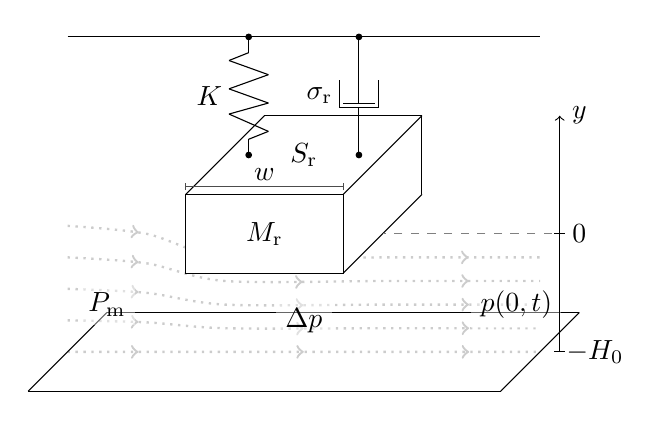
\begin{tikzpicture}
    
    \def\radius{6}; % Radius of the string (>2!)
    \pgfmathsetmacro{\reps}{3}; % How may back-and-forths in the drawing of the springs
    \def\bowSpacing{0.2};
    \def\drawingSpacing{1.5}
    \def\bowWidth{5};
    
    \def\woodWidth{1}; %>0.3
    \def\massWidth{2};
    \def\bridgeHeight{3};
    \def\bridgeWidth{4};
    \def\cornerRadius{0.15};
    \def\stringWidth{0.2};
    \pgfmathsetmacro{\tinyRadius}{\stringWidth*0.1};
    \pgfmathsetmacro{\stringWidthMinTinyRad}{((\stringWidth-(2*\tinyRadius)))*0.5};
    
    % draw airflow
    
    %draw airflow
    \def\rightAirFlow{0}; % have the right airflow bulge (1) or not (0)
    \foreach \idx in {1,...,5}
    {
        \pgfmathsetmacro{\scaleLeft}{0.5 - 0.1 * \idx};
        \ifnum\rightAirFlow=1
            \pgfmathsetmacro{\scaleRight}{0.5 - 0.1 * \idx};
        \else
            \pgfmathsetmacro{\scaleRight}{0};
        \fi
        \begin{scope}[decoration={
            markings,
            mark=between positions 0.15 and 0.85 step 0.35
         with {\arrow{>}}}
            ]
        % \node at (0, \idx) {\scale};
         \draw [gray!40, 
         xshift=-2.5cm, 
         yshift= -\idx * 0.3cm, 
         dotted, 
         line width=0.3mm, postaction={decorate}] plot [smooth, tension = 0.5] coordinates { (0,1*\scaleLeft) (1,0.75*\scaleLeft) (2,0) (4, 0) (5, 0.75*\scaleRight) (6,1*\scaleRight)} ;
         \end{scope}
    }
    % \def\scale{0.5};
    % \draw [gray, xshift=-2.5cm, yshift=-0cm] plot [smooth, tension = 0.5] coordinates { (0,1*\scale) (1,0.75*\scale) (2,0) (4, 0) (5, 0.75*\scale) (6,1*\scale)};
    % \def\scale{0.25};
    % \draw [gray, xshift=-2.5cm, yshift=-1.2cm] plot [smooth, tension = 0.5] coordinates { (0,1*\scale) (1,0.75*\scale) (2,0) (4, 0) (5, 0.75*\scale) (6,1*\scale)};
    % \def\scale{0};
    % \draw [gray, xshift=-2.5cm, yshift=-1.5cm] plot [smooth, tension = 0.5] coordinates { (0,1*\scale) (1,0.75*\scale) (2,0) (4, 0) (5, 0.75*\scale) (6,1*\scale)};
    
    \node (r0) at ( 1.0,  -0.5 ) {}; % root
    \node (s0) at ( 1.0, 0.1 ) {}; % extreme
    \node (s1) at ( 1.6, 0.1 ) {}; % extreme

    % DRAW TREE
    \fill[fill=white] (r0.center)--(s0.center)--(s1.center);
    
    % \draw plot [smooth] coordinates {(-3, -3) (-2, 2) (-1, -3};
    \node at (0,0) [rectangle,draw, fill = white, minimum height=1cm,minimum width= \massWidth cm] (Mr) {$M_\text{r}$};
    %top
    % \draw[-] (-3, 2) -- (3, 2) node[below, midway] (top) {};
    % \draw[-] (-2, 3) -- (4, 3) node[below, midway] (top) {};
    % \draw[-] (-3, 2) -- (-2, 3) node[below, midway] (top) {};
    % \draw[-] (4, 3) -- (3, 2) node[below, midway] (top) {};
    \draw[-] (-2.5, 2.5) -- (3.5, 2.5) node[below, midway] (top) {};
    %bottom
    \draw[-] (-3, -2) -- (3, -2) node[below, midway] (bottom) {};
    \draw[-] (-2, -1) -- (4, -1) node[below, midway] (bottom) {};
    \draw[-] (-3, -2) -- (-2, -1) node[below, midway] (top) {};
    \draw[-] (4, -1) -- (3, -2) node[below, midway] (top) {};

    % draw mass
    
    \draw[-] (-1, 0.5) -- (0, 1.5) node[] (left) {};

    \draw[-] (1, 0.5) -- (2, 1.5) node[] (topRight) {};

    \draw[-] (0, 1.5) -- (2, 1.5) node[] (top) {};

    \draw[-] (2, 1.5) -- (2, 0.5) node[] (right) {};

    \draw[-] (0.5 * \massWidth, -0.5) -- (2, 0.5) node[] (bottomRight) {};

    \node[rotate = 0] at (0.5, 1) (Sr) {$S_\text{r}$};

    \def\xOffset{0.3};
    % draw spring
    \filldraw[black] (-0.5 + \xOffset, 2.5) circle (1pt) node[anchor=center](topSpring){};    
    \draw[-] (-0.5 + \xOffset, 2.5) -- (-0.5 + \xOffset, 2.3);
    \draw[-] (-0.5 + \xOffset, 2.3) -- (-0.75 + \xOffset, 2.2);
    %switched these around because of the color
    \draw[-] (-0.25 + \xOffset, 2.02) -- (-0.75 + \xOffset, 1.84);
    \draw[-] (-0.75 + \xOffset, 2.2) -- (-0.25 + \xOffset, 2.02);
    \draw[-] (-0.75 + \xOffset, 1.84) -- (-0.25 + \xOffset, 1.66);
    \draw[-] (-0.25 + \xOffset, 1.66) -- (-0.75 + \xOffset, 1.52);
    \draw[-] (-0.75 + \xOffset, 1.52) -- (-0.25 + \xOffset, 1.3);
    \draw[-] (-0.25 + \xOffset, 1.3) -- (-0.5 + \xOffset, 1.2);
    \draw[-] (-0.5 + \xOffset, 1.2) -- (-0.5 + \xOffset, 1.0);
    \filldraw[black] (-0.5 + \xOffset, 1.0) circle (1pt) node[anchor=center](bottomSpring){};    
    \node at (-1 + \xOffset, 1.75) (K) {$K$};
    
    \def\dashpotHeight{-0.25}
    % draw dashpot
    \filldraw[black] (1.5 - \xOffset, 2.5) circle (1pt) node[anchor=center](topDashPot){};
    \draw[-] (1.5 - \xOffset, 2.5) -- (1.5 - \xOffset, 1.4 - \dashpotHeight);

    \draw[-] (1.3 - \xOffset, 1.4 - \dashpotHeight) -- (1.7 - \xOffset, 1.4 - \dashpotHeight);

    \draw[-] (1.25 - \xOffset, 1.7 - \dashpotHeight) -- (1.25 - \xOffset, 1.35 - \dashpotHeight);
    \draw[-] (1.75 - \xOffset, 1.35 - \dashpotHeight) -- (1.75 - \xOffset, 1.7 - \dashpotHeight);

    \draw[-] (1.25 - \xOffset, 1.35 - \dashpotHeight) -- (1.75 - \xOffset, 1.35 - \dashpotHeight);
    \draw[-] (1.5 - \xOffset, 1.35 - \dashpotHeight) -- (1.5 - \xOffset, 1.0);

    \filldraw[black] (1.5 - \xOffset, 1.0) circle (1pt) node[anchor=center](bottomDashpot){};    
    \node at (1.0 - \xOffset, 1.75) (sigma) {$\sigma_\text{r}$};
    
    
    % pressure labels
    \def\pressOffset{0.3}
    \def\backgroundOpacity{0.4}
    \node[fill = white, fill opacity=\backgroundOpacity, text opacity = 1] at (-2, -0.6 - \pressOffset) (Pm) {$P_\text{m}$};
    \node[fill = white, fill opacity=\backgroundOpacity, text opacity = 1] at (0.5, -0.8 - \pressOffset) (deltaP) {$\Delta p$};
    \node[fill = white, fill opacity=\backgroundOpacity, text opacity = 1] at (3.2, -0.6 - \pressOffset) (p) {$p(0,t)$};

    
    % y and H0
    \def\axisLineWidth{0.07};
    \draw[dashed, color = gray] (3.65, 0) -- (1.5, 0);
    \node at (4, 1.5) {$y$};
    
    \draw[->] (3.75, -1.5) -- (3.75, 1.5);
    \node at (4, 0) {$0$};
    \draw (3.75 - \axisLineWidth, 0) -- (3.75 + \axisLineWidth, 0) {};

    \draw (3.75 - \axisLineWidth, -1.5) -- (3.75 + \axisLineWidth, -1.5) {};
    \node at (4.2, -1.5) {$-H_0$};
    
    % width
    \draw[black!70] (-1, 0.6) -- (1, 0.6) {};
    \draw[black!70] (-1, 0.55) -- (-1, 0.65) {};
    \draw[black!70] (1, 0.55) -- (1, 0.65) {};
    \node at (0, 0.75) (w) {$w$};
% \begin{scope}[very thick,decoration={
%     markings,
%     mark=at position 0.5 with {\arrow{>}}}
%     ] 
%     \draw[postaction={decorate}] (-4,0)--(4,0);
% \end{scope}
    
    \end{tikzpicture}
    \caption{Lipsystem with the equilibrium at 0 and the distance from the lower lip $H_0$.}
    \label{fig:lipSystem}
\end{figure}
This pressure difference causes a volume flow velocity following the Bernoulli equation
\begin{equation}
    U_\text{B} = w[y + H_0]_+\text{sgn}(\Delta p) \sqrt{\frac{2|\Delta p|}{\rho_0}},
\end{equation}
with effective lip-reed width $w$ (m), static equilibrium separation $H_0$ (m) and $[x]_+ = 0.5 (x + |x|)$ describes the ``positive part of`''. Notice that when $y + H_0 \leq 0$, the lips are closed and the volume velocity $U_\text{B}$ is 0. Another volume flow is generated by the lip reed itself according to
\begin{equation}
    U_\text{r} = S_\text{r} \frac{dy}{dt}.
\end{equation}
Assuming that the volume flow velocity is conserved we define the total air volume entering the system is defined as
\begin{equation}
    S(0)v(0,t) = U_\text{B}(t) + U_\text{r}(t).
\end{equation}

\subsection{Discrete Time}
\def\nph{}
\def\nphSys{n+1/2}

Placing $y$, $\Delta p$, and thereby $U_\text{B}$ and $U_\text{r}$ on the interleaved temporal grid (but on the non-interleaved spatial grid), we discretise the equations above to get the following system
\begin{subnumcases}{\label{eq:discreteLipSystem}}
    M_\text{r}\delta_{tt}y^{\nphSys} & $= -M_\text{r}\omega_0^2\mu_{t\cdot}y^{\nphSys}-M_\text{r}\sigma_\text{r}\delta_{t\cdot}y^{\nphSys} + S_\text{r}\Delta p^{\nphSys}$\label{eq:discReed}\\
    \Delta p^{\nphSys} & $= P_\text{m} - \mu_{t+}p_0^n$\label{eq:pDiff}\\
    U_\text{B}^{\nphSys} & $= w[y^{\nphSys}+H_0]_+\text{sgn}(\Delta p^{\nphSys})\sqrt{\frac{2|\Delta p^{\nphSys}|}{\rho_0}}$\label{eq:bernoulli}\\
    U_\text{r}^{\nphSys} & $= S_\text{r}\delta_{t\cdot}y^{\nphSys}$\label{eq:Ur}\\
    \mu_{x-}(S_{1/2}v_{1/2}^{\nphSys}) &$= U_\text{B}^{\nphSys} + U_\text{r}^{\nphSys}$\label{eq:UbUr}
\end{subnumcases}
In the following we will suppress the superscript $n+1/2$ for the aforementioned variables. Expanding and solving \eqref{eq:discReed} for $y^{n+3/2}$ yields
\begin{align}
    \left(1 + \frac{\omega_0^2 k^2}{2} + \frac{\sigma_\text{r} k}{2}\right)y^{n+3/2} &= 2 y^{n+1/2} - \left(1 + \frac{\omega_0^2 k^2}{2} - \frac{\sigma_\text{r} k}{2}\right) y^{n-1/2} + \frac{S_\text{r} k^2}{M_\text{r}} \Delta p^{\nph}\nonumber\\
    \alpha_\text{r}y^{n+3/2} &= 4y^{n+1/2} + \beta_\text{r}y^{n-1/2} + \xi_\text{r}\Delta p^{\nph}
\end{align}
where
\begin{equation}
    \alpha_\text{r} = 2 + \omega_0^2k^2 + \sigma_\text{r} k\ , \qquad \beta_\text{r} =  \sigma_\text{r} k - 2 - \omega_0^2 k^2\ , \qquad \text{and} \qquad \xi_\text{r} = \frac{2 S_\text{r}k^2}{M_\text{r}}.
\end{equation}
\subsubsection{Obtaining $\Delta p$}\label{sec:obtainingDeltaP}
With all other parameters user-defined, the only unknown in our system is now $\Delta p^{\nph}$. Using the following identities
\begin{equation}
    \delta_{tt} = \frac{2}{k}(\delta_{t\cdot} - \delta_{t-}), \quad \text{and} \quad \mu_{t\cdot} = k\delta_{t\cdot} + e_{t-}
\end{equation}
where $e_{t-}$ is a backwards time-shift of one sample (so $e_{t-}y^{n+1/2} = y^{n-1/2}$) we can rewrite \eqref{eq:discReed} to
\begin{gather}
    \frac{2}{k} (\delta_{t\cdot} - \delta_{t-})y^{\nph} = -\omega_0^2(k\delta_{t\cdot} + e_{t-})y^{\nph} - \sigma_\text{r}\delta_{t\cdot} y^{\nph} + \frac{S_\text{r}}{M_\text{r}}\Delta p^{\nph}\nonumber\\
    a_1\delta_{t\cdot}y^{\nph} - a_2\Delta p^{\nph} - a_3^n = 0,\label{eq:preAEquation}
\end{gather}
where
\begin{equation}\label{eq:aCoeffs}
    a_1 = \frac{2}{k} + \omega_0^2k + \sigma_\text{r} \geq 0, \quad a_2 = \frac{S_\text{r}}{M_\text{r}} \geq 0\ , \quad \text{and} \quad a_3^n = \left(\frac{2}{k} \delta_{t\cdot} - \omega_0^2e_{t-}\right)y^{\nph}\ .
\end{equation}
Note that because $a_1$ and $a_2$ are calculated solely from non-negative parameters we can apply the condition that these are greater than or equal to 0. The same will be done for other coefficients below.
We can substitute Eq. \eqref{eq:Ur} into Eq. \eqref{eq:preAEquation}
\begin{equation}
    \frac{a_1}{S_\text{r}}U_\text{r}^{\nph} - a_2 \Delta p^{\nph} - a_3^n = 0
\end{equation}
and consequently \eqref{eq:UbUr} to get
\begin{equation}\label{eq:aEquation}
    \frac{a_1}{S_\text{r}}\left(\mu_{x-}(S_{1/2}v_{1/2}^{\nph}) - U_\text{B}^{\nph}\right) - a_2 \Delta p^{\nph} - a_3^n = 0
\end{equation}
%
To get a definition for $\mu_{x-}(S_{1/2}v_{1/2}^{\nph})$, we include the expression for Webster's equation at $l=0$
\begin{equation}
    \frac{\bar S_0}{\rho_0 c^2}\delta_{t+}p_0^n = -\delta_{x-}(S_{1/2}v_{1/2}^{\nph}),
\end{equation}
which, using the following identity (derived from Eq. (2.7d) from \cite{Bilbao2009})
\begin{equation}\label{eq:identity}
    \delta_{x\pm} = \pm\frac{2}{h}(\mu_{x\pm} - 1),
\end{equation} 
can be rewritten to
\begin{equation}
    \frac{\bar S_0}{\rho_0 c^2}\delta_{t+}p_0^n = \frac{2}{h} \left(\mu_{x-}(S_{1/2}v_{1/2}^{\nph})-S_{1/2}v_{1/2}^{\nph}\right).
\end{equation}
Then using the same identity \eqref{eq:identity} but for $\delta_{t+}$ we get
\begin{equation}
    \frac{2\bar S_0}{\rho_0 c^2k}(\mu_{t+}p_0^n-p_0^n) = \frac{2}{h} \left(\mu_{x-}(S_{1/2}v_{1/2}^{\nph})-S_{1/2}v_{1/2}^{\nph}\right).
\end{equation}
Using Eq. \eqref{eq:pDiff} we can rewrite this to
\begin{align}
    \frac{\bar S_0h}{\rho_0 c^2k}(P_\text{m} - \Delta p^{\nph}-p_0^n) &= \frac{2}{h} \left(\mu_{x-}(S_{1/2}v_{1/2}^{\nph})-S_{1/2}v_{1/2}^{\nph}\right).\nonumber\\
    \mu_{x-}(S_{1/2}v_{1/2}^{\nph}) &= b_1^n - b_2\Delta p^{\nph}\label{eq:bEquation}
\end{align}
where
\begin{equation}\label{eq:bCoeffs}
    b_1^n = S_{1/2}v_{1/2}^{\nph} + \frac{\bar S_0h}{\rho_0 c^2k} (P_\text{m} - p_0^n), \quad \text{and} \quad b_2 = \frac{\bar S_0h}{\rho_0 c^2k} \geq 0\ .
\end{equation}
We can then substitute Eqs. \eqref{eq:bEquation} and \eqref{eq:bernoulli} into Eq. \eqref{eq:aEquation} to get
\begin{gather}
    \frac{a_1}{S_\text{r}}\left(b_1^n - b_2\Delta p^{\nph} - w[y^{\nph}+H_0]_+\text{sgn}(\Delta p^{\nph})\sqrt{\frac{2|\Delta p^{\nph}|}{\rho_0}}\right) - a_2 \Delta p^{\nph} - a_3^n = 0,\nonumber\\
    - w[y^{\nph}+H_0]_+\text{sgn}(\Delta p^{\nph})\sqrt{\frac{2|\Delta p^{\nph}|}{\rho_0}} - b_2\Delta p^{\nph} - \frac{a_2S_\text{r}}{a_1} \Delta p^{\nph} + b_1^n - \frac{a_3^nS_\text{r}}{a_1} = 0,\nonumber\\
    -c_1^n\text{sgn}(\Delta p^{\nph})\sqrt{|\Delta p^{\nph}|} - c_2\Delta p^{\nph} + c_3^n = 0\label{eq:cEquation}
\end{gather}
where
\begin{equation}\label{eq:cCoeffs}
    c_1^n = w[y^{\nph} + H_0]_+\sqrt{\frac{2}{\rho_0}} \geq 0, \quad c_2 = b_2 + \frac{a_2S_\text{r}}{a_1} \geq 0, \quad \text{and}\quad c_3^n = b_1^n - \frac{a_3^nS_\text{r}}{a_1}\ .
\end{equation}
We can then divide Eq. \eqref{eq:cEquation} by $-\text{sgn}(\Delta p^{\nph})$ to get a quadratic equation in $\sqrt{|\Delta p^{\nph}|}$
\begin{equation}
    c_2|\Delta p^{\nph}| + c_1^n\sqrt{|\Delta p^{\nph}|} - \frac{c_3^n}{\text{sgn}(\Delta p^{\nph})} = 0.
\end{equation}
Now, as we know that $c_1^n, c_2 \geq 0$, for any real solutions to exist the following must be true
\begin{equation}\label{eq:sgnEquality}
    \text{sgn}(c_3^n) = \text{sgn}(\Delta p^{\nph}) \quad \Longrightarrow \quad \frac{c_3^n}{\text{sgn}(\Delta p^{\nph})} = |c_3^n|.
\end{equation}
Now we can solve for $\sqrt{|\Delta p^{\nph}|}$:
\begin{equation}
    \sqrt{|\Delta p^{\nph}|} = \frac{-c_1^n \pm \sqrt{(c^n_1)^2+4c_2|c_3^n|}}{2c_2}\ .
\end{equation}
As $\sqrt{(c_1^n)^2 + 4c_2|c_3^n|} \geq c_1^n$, we can only guarantee that the solution is positive if we take the positive solution the square root. Furthermore, using Eq. \eqref{eq:sgnEquality} we can solve for the pressure difference
\begin{equation}\label{eq:pressureDiff}
    \Delta p^{\nph} = \text{sgn}(c_3^n)\left(\frac{-c_1^n + \sqrt{(c^n_1)^2+4c_2|c_3^n|}}{2c_2}\right)^2.
\end{equation}
This we can then apply to the update of the lip reed in Eq. \eqref{eq:discReed}. 

\subsubsection{Coupling to the tube}
To couple the reed to the tube, we take Eq. \eqref{eq:pressureUpdate} at $l=0$ and rewrite it to
\begin{equation}
    p^{n+1}_0 = p_0^n - \frac{\rho_0c\lambda}{\bar S_0}\left(-2\mu_{x-}(S_{1/2}v_{1/2}^{\nph}) + 2 S_{1/2}v_{1/2}^{\nph}\right),
\end{equation}
and substitute Eq. \eqref{eq:UbUr} to get
\begin{equation}\label{eq:pressureCoupled}
    p^{n+1}_0 = p_0^n - \frac{\rho_0c\lambda}{\bar S_0}\left(-2(U_\text{B}^{\nph} + U_\text{r}^{\nph}) + 2 S_{1/2}v_{1/2}^{\nph}\right).
\end{equation}
\subsection{Energy analysis}
We start by multiplying Eq. \eqref{eq:discReed} by $\delta_{t\cdot}y$ (superscript $n+1/2$ is again suppressed):
\begin{alignat}{2}
    &\xLeftrightarrow{\mystrut\ \text{Eq. \eqref{eq:pDiff}}\ }\qquad\qquad\qquad\qquad\qquad\qquad\quad M_\text{r}\delta_{t\cdot}y^{\nph}\delta_{tt}y^{\nph} + M_\text{r}\omega_0^2\delta_{t\cdot}y^{\nph}\mu_{t\cdot}y^{\nph} + M_\text{r} \sigma_\text{r}(\delta_{t\cdot}y^{\nph})^2 - S_\text{r}\delta_{t\cdot}y^{\nph}\Delta p^{\nph} &&= 0,\nonumber\\[-5pt]
    &\xLeftrightarrow{\mystrut\ \text{Eqs. \eqref{eq:Ur} \& \eqref{eq:UbUr}}\ } \qquad \ \: M_\text{r}\delta_{t\cdot}y^{\nph}\delta_{tt}y^{\nph} + M_\text{r}\omega_0^2\delta_{t\cdot}y^{\nph}\mu_{t\cdot}y^{\nph} + M_\text{r} \sigma_\text{r}(\delta_{t\cdot}y^{\nph})^2 - \left(\mu_{x-}(S_{1/2}v_{1/2})-U_\text{B}\right)\Delta p^{\nph} &&= 0,\nonumber\\[-5pt]
    &\xLeftrightarrow{\mystrut\ \text{Eq. \eqref{eq:pDiff}}\ } \quad M_\text{r}\delta_{t\cdot}y^{\nph}\delta_{tt}y^{\nph} + M_\text{r}\omega_0^2\delta_{t\cdot}y^{\nph}\mu_{t\cdot}y^{\nph} + M_\text{r} \sigma_\text{r}(\delta_{t\cdot}y^{\nph})^2 + U_\text{B}\Delta p^{\nph}-\mu_{x-}(S_{1/2}v_{1/2})(P_\text{m} - \mu_{t+}p_0) &&= 0,\nonumber
\end{alignat}
\vspace{-5pt}\\
Recalling that the energy of the tube $\delta_{t+}\mathfrak{h}_\text{t} = \mathfrak{b}_\text{r} + \mathfrak{b}_\text{l}$ and $\mathfrak{b}_\text{l} = -(\mu_{t+}p_0)\mu_{x-}(S_{1/2}v_{1/2})$ we get, assuming that $\mathfrak{b}_\text{r} = 0$\vspace{-5pt}
\begin{alignat}{2}
    &\xLeftrightarrow{\mystrut\ \text{Eq. \eqref{eq:firstOrderLeftBoundary}}\ }\qquad\ \  M_\text{r}\delta_{t\cdot}y^{\nph}\delta_{tt}y^{\nph} + M_\text{r}\omega_0^2\delta_{t\cdot}y^{\nph}\mu_{t\cdot}y^{\nph} + M_\text{r} \sigma_\text{r}(\delta_{t\cdot}y^{\nph})^2 + U_\text{B}\Delta p^{\nph}-\mu_{x-}(S_{1/2}v_{1/2})P_\text{m} + \delta_{t+}\mathfrak{h}_\text{t} &&= 0,\nonumber
\end{alignat}
Then we arrive at the following energy balance
\begin{equation}
    \delta_{t+}\left(\mathfrak{h}_\text{t}+\mathfrak{h}_\text{r}\right) + \mathfrak{Q}_\text{r} + \mathfrak{p}_\text{r} = 0
\end{equation}
where
\begin{gather}
    \mathfrak{h}_\text{r} = \frac{M_\text{r}}{2}\left((\delta_{t-}y)^2+\omega_0^2\mu_{t-}(y^2)\right) \geq 0\\
    \mathfrak{Q}_\text{r} = M_\text{r}\sigma_\text{r}(\dtd y)^2 + U_\text{B}\Delta p^{\nph} \geq 0\\
    \mathfrak{p}_\text{r} = -(U_\text{B} + U_\text{r})P_\text{m}
\end{gather}

\subsection{Adding lip collision}
We can use \SWcomment[Michele's tricks] to add a non-linear collision to the lip. As the collision happens at the interleaved temporal grid, we move the potential half a time step forward. We extend Eq. \eqref{eq:discReed} to be
\begin{equation}
    M_\text{r}\delta_{tt}y^{\nph} = -M_\text{r}\omega_0^2\mu_{t\cdot}y^{\nph}-M_\text{r}\sigma_\text{r}\delta_{t\cdot}y^{\nph} + S_\text{r}\Delta p^{\nph} + \psi^{n+1/2}(\psi^{n+1/2})', 
\end{equation}
which, when using $\mu_{t+}\psi^n = \psi^{n+1/2}$, we can then rewrite to
\begin{equation}
    M_\text{r}\delta_{tt}y^{\nph} = -M_\text{r}\omega_0^2\mu_{t\cdot}y^{\nph}-M_\text{r}\sigma_\text{r}\delta_{t\cdot}y^{\nph} + S_\text{r}\Delta p^{\nph} + (\mu_{t+}\psi^n)g^{n+1/2} 
\end{equation}
with
\begin{equation}\label{eq:gnph}
    g^{n+1/2} = \frac{\delta_{t+}\psi^n}{\delta_{t\cdot}\eta^{n+1/2}}\ ,
\end{equation}
distance between the lips
\begin{equation}\label{eq:etaBarrier}
    \eta^{n+1/2} = b - y^{n+1/2}
\end{equation}
and the location of the lower lip $b = -H_0$. Rewriting Eq. \eqref{eq:gnph} to
\begin{equation}\label{eq:rewrittenPsi}
    \delta_{t+}\psi^n = g^{n+1/2}\delta_{t\cdot}\eta^{n+1/2}
\end{equation}
and using identity
\begin{equation}
    \mu_{t+}\psi^n = \frac{k}{2}\delta_{t+}\psi^n + \psi^n
\end{equation} 
we arrive at
\begin{equation}
    M_\text{r}\delta_{tt}y^{\nph} = -M_\text{r}\omega_0^2\mu_{t\cdot}y^{\nph}-M_\text{r}\sigma_\text{r}\delta_{t\cdot}y^{\nph} + S_\text{r}\Delta p^{\nph} + \left(\frac{k}{2}g^{n+1/2}\delta_{t\cdot}\eta^{n+1/2} + \psi^n\right)g^{n+1/2},
\end{equation}
where $g^{n+1/2}$ can be analytically obtained through 
\begin{equation}\label{eq:gAnalytic}
    g^{n+1/2} = (\psi^{n+1/2})'\bigg\rvert_{\eta = \eta^{n+1/2}} = \sqrt{\frac{K_\text{c}(\alpha_\text{c} + 1)}{2}}[\eta^{n+1/2}]_+^{\frac{\alpha_\text{c}-1}{2}},
\end{equation}
with collision stiffness $K_\text{c}$ (in N/m if $\alpha_\text{c} = 1$) and non-linear collision coefficient $\alpha_\text{c}$. Finally, because the barrier is static and below $y$ through \eqref{eq:etaBarrier}, this implies that
\begin{equation}\label{eq:etaNegY} 
    \delta_{t\cdot}\eta = -\delta_{t\cdot}y
\end{equation}
and we can solve for $y^{n+3/2}$ (suppressing the $n+1/2$ superscript for) $g$
\begin{align}
    \frac{1}{k^2}(y^{n+3/2} - 2y^{n+1/2} + y^{n-1/2}) = &-\frac{\omega_0^2}{2}(y^{n+3/2}+y^{n-1/2})-\frac{\sigma_\text{r}}{2k}(y^{n+3/2}-y^{n-1/2})\nonumber \\
    &+ \frac{S_\text{r}}{M_\text{r}}\Delta p^{\nph}  -\frac{g^2}{4M_\text{r}}(y^{n+3/2}-y^{n-1/2}) + \frac{g}{M_\text{r}}\psi^n\nonumber\\
    \left(2 + \omega_0^2 k^2 + \sigma_\text{r} k + \frac{g^2k^2}{2M_\text{r}}\right) y^{n+3/2} &= 4y^{n+1/2}+ \left(\sigma_\text{r}k - 2 - \omega_0^2k^2 + \frac{g^2k^2}{2M_\text{r}}\right) y^{n-1/2}\nonumber\\
    &+ \frac{2S_\text{r}k^2}{M_\text{r}}\Delta p^{\nph} + \frac{2gk^2}{M_\text{r}}\psi^n\nonumber.
\end{align}
Finally we get
\begin{equation}\label{eq:lipUpdateWithCollision}
    \alpha_\text{r}y^{n+3/2} = 4 y^{n+1/2} + \beta_\text{r}y^{n-1/2} + \xi_\text{r}\Delta p + 4\psi^n\gamma_\text{r}
\end{equation}
with
\begin{gather}
    \alpha_\text{r} = 2 + \omega_0^2 k^2 + \sigma_\text{r} k + g\gamma_\text{r}, \quad \beta_\text{r} = \sigma_\text{r}k - 2 - \omega_0^2k^2 + g\gamma_\text{r}, \nonumber \\[10pt]
    \xi_\text{r} = \frac{2S_\text{r}k^2}{M_\text{r}}, \quad \text{and} \quad \gamma_\text{r} = \frac{gk^2}{2M_\text{r}}\ .\nonumber
\end{gather}
For calculating $\Delta p$ we follow the same steps as in Section \ref{sec:obtainingDeltaP} to get
\begin{gather}
    \frac{2}{k} (\delta_{t\cdot} - \delta_{t-})y^{\nph} = -\omega_0^2(k\delta_{t\cdot} + e_{t-})y^{\nph} - \sigma_\text{r}\delta_{t\cdot} y^{\nph} + \frac{S_\text{r}}{M_\text{r}}\Delta p^{\nph} + \frac{1}{M_\text{r}}\left(-\frac{k}{2}g\delta_{t\cdot}y+\psi^n\right)g\nonumber\\
    a_1\delta_{t\cdot}y^{\nph} - a_2\Delta p^{\nph} - a_3^n = 0,\label{eq:preAEquation}
\end{gather}
with 
\begin{equation}\label{eq:aColCoeffs}
    a_1^n = \frac{2}{k} + \omega_0^2k + \sigma_\text{r} + \frac{g^2k}{2M_\text{r}} \geq 0, \quad a_2 = \frac{S_\text{r}}{M_\text{r}} \geq 0\ , \quad \text{and} \quad a_3^n = \left(\frac{2}{k} \delta_{t\cdot} - \omega_0^2e_{t-}\right)y^{\nph} + \frac{g}{M_\text{r}}\psi^n\ .
\end{equation}
Note that $a_1^n$ is now time-dependent through $g$ but remains non-negative. The rest of the variables and process in Section \ref{sec:obtainingDeltaP} are unchanged.

Knowing $y^{n+3/2}$ we can calculate $\psi^{n+1}$ through Eqs. \eqref{eq:etaBarrier} and \eqref{eq:rewrittenPsi} with
\begin{equation}\label{eq:psiUpdate}
    \psi^{n+1} = \psi^n - \frac{g}{2}\left(y^{n+3/2} - y^{n-1/2}\right)
\end{equation}
\subsubsection{Energy}
The added energy to the system can be calculated by multiplying the added term with $\delta_{t\cdot}y$
\begin{align}
    \delta_{t+}(\mathfrak{h}_\text{t}+\mathfrak{h}_\text{r}) + \mathfrak{Q}_\text{r} + \mathfrak{p}_\text{r}&-(\mu_{t+}\psi^n) \frac{\delta_{t+}\psi^n}{\delta_{t\cdot}\eta^{n+1/2}}(\delta_{t\cdot}y^{n+1/2}) = 0\nonumber\\[-5pt]
    \xLeftrightarrow{\mystrut\ \text{Eq. \eqref{eq:etaNegY}}\ }\quad \hdots &+ (\mu_{t+}\psi^n) (\delta_{t+}\psi^n) = 0\nonumber\\
    \hdots &+ \frac{1}{2k}(\psi^{n+1}+\psi^n)(\psi^{n+1} - \psi^n)=0\nonumber\\
    \hdots  &+\frac{1}{2k}((\psi^{n+1})^2 - (\psi^n)^2)=0\nonumber\\
    \hdots &+ \frac{1}{2}\delta_{t+}\left((\psi^n)^2\right) = 0\nonumber\\
    \delta_{t+}(\mathfrak{h}_\text{t}+\mathfrak{h}_\text{r} + \mathfrak{h}_\text{c}) &+ \mathfrak{Q}_\text{r} + \mathfrak{p}_\text{r} = 0
\end{align}
with
\begin{equation}
    \mathfrak{h}_\text{c} = \frac{(\psi^n)^2}{2 }\nonumber
\end{equation}

\section{Implementation}
The order of calculation then becomes:
\begin{algorithm}[ht]
\centering
\fbox{\parbox{0.9\linewidth}{
\setstretch{1.5}
 \While{application is running}{
 \vspace{0.15cm}
 \begin{minipage}[c]{0.48\linewidth}
1. Calculate $v^{n+1/2}$\\
2. Calculate $\eta^{n+1/2}$\\
3. Calculate $g^{n+1/2}$\\
4. Update $a_1^n, a_2, a_3^n, b_1^n, b_2, c_1^n, c_2$ and $c_3$\\
5. Calculate $\Delta p^{n+1/2}$\\
6. Calculate $y^{n+3/2}$\\
7. Calculate $\psi^{n+1}$\\
8. Calculate $p^{n+1}$\\
\vspace{0.15cm}9. Update states\\
\end{minipage}
\hspace{0.05cm}
\begin{minipage}[c]{0.42\linewidth}
(Eq. \eqref{eq:velocityUpdate})\\
(Eq. \eqref{eq:etaNegY})\\
(Eq. \eqref{eq:gAnalytic})\\
(Eqs. \eqref{eq:aColCoeffs}, \eqref{eq:bCoeffs} and \eqref{eq:cCoeffs})\\
(Eq. \eqref{eq:pressureDiff})\\
(Eq. \eqref{eq:lipUpdateWithCollision})\\
(Eq. \eqref{eq:psiUpdate})\\
(Eqs. \eqref{eq:pressureUpdate} and \eqref{eq:pressureCoupled})\\
$v^{n-1/2} = v^{n+1/2}$, $p^{n-1} = p^{n+1}$, \\
$\psi^n = \psi^{n+1}$
\end{minipage}
 }
 }
 }
 \vspace{0.2cm}
 \caption{Pseudocode showing the order of calculation. \label{alg:calcOrder}}
\end{algorithm}
\section{Time-varying System}
The PDE for the time-varying version of Webster's equation is (Eq. (9.23) in \cite{Bilbao2009})
\begin{equation}
     \partial_t(S\partial_t\Psi) = c^2 \partial_x(S\partial_x\Psi).
\end{equation}
which can be discretised as (right below Eq. (9.23) in \cite{Bilbao2009})
\begin{equation}
    \delta_{t+}\big((\mu_{t-}\bar S_l^n)(\delta_{t-}\Psiln)\big) = c^2\dxp\big((\muTT \Sm^n)(\dxm\Psiln)\big)
\end{equation}
The update scheme for this time varying system can be written as
\begin{equation}
    \begin{aligned}
        (\mu_{t+}\bar S_l^n)\Psinp &= \Big(2 \mu_{tt}\bar S_l^n -  \lambda^2(\muTT \Sp^n + \muTT \Sm^n)\Big) \Psiln \\
        &+ \lambda^2 \Big((\muTT \Sp^n)\Psilp + (\muTT\Sm)\Psilm\Big) - (\mu_{t-}\bar S_l^n)\Psinm
    \end{aligned}
\end{equation}

\section{Excitation}
To excite the system, an input impedance can be defined as follows
\begin{equation}
\delta_{x\cdot}\Psi_0^n = -v_\text{in}^n.
\end{equation} 
Rewriting to
\begin{equation}
    \frac{1}{2h}(\Psi_1^n-\Psi_{-1}^n) = -v_\text{in}^n \quad \Rightarrow \quad \Psi_{-1}^n = \Psi_1^n + 2hv_\text{in}^n
\end{equation}
and substituting this in Eq. \eqref{eq:webstersUpdateEq} at $l=0$ yields
\begin{align}
    \Psi_0^{n+1}&= 2(1-\lambda^2)\Psi_0^n-\Psi_0^{n-1}+ \frac{\lambda^2S_{1/2}}{\bar S_0}\Psi_1^n + \frac{\lambda^2S_{-1/2}}{\bar S_0}\Psi_1 + \frac{2h\lambda^2S_{-1/2}}{\bar S_0}v_\text{in}^n,\nonumber\\
    \Psi_0^{n+1}&= 2(1-\lambda^2)\Psi_0^n-\Psi_0^{n-1}+ \frac{2\lambda^2(S_{1/2}+S_{-1/2})}{S_{1/2}+S_{-1/2}}\Psi_1^n+ \frac{2h\lambda^2S_{-1/2}}{\bar S_0}v_\text{in}^n,\nonumber\\
    \Psi_0^{n+1}&= 2(1-\lambda^2)\Psi_0^n-\Psi_0^{n-1}+ 2\lambda^2\Psi_1^n+ \frac{2h\lambda^2S_{-1/2}}{\bar S_0}v_\text{in}^n,
\end{align}
which is identical to Eq. (19.58) in \cite{Bilbao2018}.
\section{Damping}
As said in \cite{Bilbao2013}, a fractional derivative can be used for viscothermal damping. This, in discrete time can be approximated using the bilinear transform (or Tustin's transformation).

Following \cite{Chen2002}:
\begin{equation}
    (\omega(\z))^r = \left(\frac{2}{k}\right)^r \left(\frac{1-\z}{1+\z}\right)^r.
\end{equation}
Then, if we consider $r = 3$:
\begin{equation}
    \begin{aligned}
    (\omega(\z))^3 &= \left(\frac{2}{k}\right)^3\left(\frac{(1-\z)^3}{(1+\z)^3}\right)\\
    &= \left(\frac{2}{k}\right)^3\left(\frac{1-\z-2\z+2z^{-2}+z^{-2}-z^{-3}}{1+\z+2\z+2z^{-2}+z^{-2}+z^{-3}}\right)\\
    &= \left(\frac{2}{k}\right)^3\left(\frac{1-3\z+3z^{-2}-z^{-3}}{1+3\z+3z^{-2}+z^{-3}}\right)
    \end{aligned}
\end{equation}
We can do the same if we follow Eq. (2) from \cite{Chen2002} with $n=3$:
\begin{equation}
    \begin{aligned}
    (\omega(\z))^3 &= \left(\frac{2}{k}\right)^3\frac{A_3(\z,3)}{A_3(\z,-3)}\\
    &= \left(\frac{2}{k}\right)^3\frac{-\frac{1}{3}3z^{-3}+\frac{1}{3}3^2z^{-2}-3\z+1}{-\frac{1}{3}(-3)z^{-3}+\frac{1}{3}(-3)^2z^{-2}-(-3)\z+1}\\
    &=\left(\frac{2}{k}\right)^3\frac{-z^{-3}+3z^{-2}-3\z+1}{z^{-3}+3z^{-2}+3\z+1},
    \end{aligned}
\end{equation}
which is equivalent to (19).

\subsection{Muir-recursion}
The Muir-recursion is described as
\begin{equation}\label{eq:muir}
    A_n(\z,r) = A_{n-1}(\z,r) -c_nz^nA_{n-1}(z,r) \quad \text{with} \quad A_0(z^{-1},r) = 1
\end{equation}
and
\begin{equation}
    c_n=
    \begin{cases}
    r/n & n \text{ is odd},\\
    0 & n \text{ is even.}
    \end{cases}
\end{equation}
If we let $n=3$ we get
\begin{equation}
    \begin{aligned}
        A_3(\z,r)&= A_2(\underbrace{(\z)^{-1}}_{z},r) - \frac{r}{3}(\z)^3A_2(\z,r)\\
        &= A_1((z)^{-1},r) - \frac{r}{3}z^{-3}A_1((\z)^{-1},r)\\
        &= A_0((\z)^{-1},r) - r(\z)^1A_0(\z,r)-\frac{r}{3}z^{-3}\left(A_0((z)^{-1},r)-rz^1A_0(z,r)\right)\\
        &(if\ A_0(z,r) = 1)\\
        &=1-r\z-\frac{r}{3}z^{-3}\left(1-rz\right)\\
        &=1-r\z+\frac{r^2}{3}z^{-2}-\frac{r}{3}z^{-3}
    \end{aligned}
\end{equation}
\subsection{Implementation of Muir-recursion}
Classes and member variables

\begin{itemize}
    \item \texttt{Z}
    \subitem \texttt{\type[double] coeff}
    \subitem \texttt{\type[int] power}
    \item \texttt{Equation\textless M\textgreater}
    \subitem \texttt{\type[std::vector\textless M\textgreater] zs} (of length M+1)
    \subitem \texttt{\type[int] zSign} (that only takes the values $-1$ and $1$).
\end{itemize}

There are a few observations that I made that helped the implementation
\begin{itemize}
    \item 
\end{itemize}

\subsubsection{The \texttt{swapCoeffs (\type[int] amount)} function}
This function is called when a \texttt{Z} is multiplied onto an \texttt{Equation}, i.e. the last term of Eq. \eqref{eq:muir} ($z^nA_{n-1}(z,r)$). I observed that in this term of the recursion the following relationship is true:
\begin{equation}\label{eq:relationship}
    \text{For any } z^p\cdot A(z,r), \quad  p = p_{A+} + 2\cdot\text{sgn}(p_{A+}),
\end{equation}
where $p_{A+}$ is the largest  power whether positive or negative present in $A$ (i.e. furthest away from 0). For example, the following could occur in the recursion:
\begin{equation}\label{eq:recursionExample}
    z^3 (A_1(z^{-1}, r)) = z^3(1 - rz^{-1}) = z^3 - rz^2.
\end{equation}
In this case $p_{A+} = -1$, and $p = 3$ (as can also be seen from the relationship in \eqref{eq:relationship}).
\\
\\
\noindent Now, the implementation of this allows us to swap coefficients of the \texttt{Z}'s in the z-vector around
\begin{equation}
\text{swap-around index} = |p| / 2,
\end{equation}
where $p$ is -- again -- the power of the $z$ multiplied onto the equation. As this power is always odd, the swap-around index is an integer-and-a-half. For the above example, the \texttt{Z} is $z^3$ and the \texttt{Equation} is $A_1(z^{-1},r) = 1-rz^{-1}$. The coefficients-vector of the \texttt{Equation}, \texttt{$\{$1, -r, 0, 0$\}$} (with negative powers) can now be flipped around index abs(3) / 2 = 1.5, so between index $1$ and $2$. If this is done and the signs of the powers of the \texttt{Z}'s in the vector are flipped, the coefficient-vector of the solution looks like \texttt{$\{$0, 0, -r, 1$\}$} (with positive powers), which is shown in the Eq. \eqref{eq:recursionExample}, i.e. $0z^0+0z^1-rz^2+1z^3$.
     
\bibliographystyle{plain}
\bibliography{bibliography}
\appendix
\def\Psinplp{\Psi_{l+1}^{n+1}}
\def\Psinmlp{\Psi_{l+1}^{n-1}}

\section{Derivations}
\subsection{Webster's Update Equation}\label{app:webstersUpdateEq}

\begin{align}
    \frac{\Sbar}{k^2}(\Psinp - 2\Psiln+\Psinm) &= c^2\left((\dxp \Sm)(\mup \dxm \Psiln) + (\mup \Sm)(\dxp \dxm \Psiln)\right)\nonumber\\
    \Psinp - 2\Psiln+\Psinm &= \frac{c^2k^2}{\Sbar}\bigg(\frac{1}{h}(\Sp - \Sm)\frac{1}{2h}\overbrace{(\Psilp -\Psilm)}^{\mup\dxm\Psiln = \delta_{x\cdot}\Psiln}\nonumber\\
    &\qquad\qquad+\frac{1}{2}(\Sp + \Sm)\frac{1}{h^2}(\Psilp-2\Psiln+\Psilm)\bigg)\nonumber\\
    \Psinp &= 2\Psiln-\Psinm + \overbrace{\frac{\lambda^2}{2\Sbar}}^{\lambda = \frac{ck}{h}}\Big(\Sp\Psilp - \Sp\Psilm - \Sm\Psilp + \Sm\Psilm \nonumber\\
    &+ \Sp\Psilp + \Sp\Psilm + \Sm\Psilp + \Sm\Psilm - 2 (\Sp + \Sm)\Psiln\Big)\nonumber\\
    \Psinp &= 2\Psiln-\Psinm+ \frac{\lambda^2}{2\Sbar}\Big(2\Sp\Psilp + 2\Sm\Psilm - 4\Sbar\Psiln\Big)\nonumber\\
    \Psinp &= 2\Psiln-\Psinm+ \frac{\lambda^2\Sp}{\Sbar}\Psilp + \frac{\lambda^2\Sm}{\Sbar}\Psilm - 2\lambda^2\Psiln\nonumber\\
    \Psinp &= 2(1-\lambda^2)\Psiln-\Psinm+ \frac{\lambda^2\Sp}{\Sbar}\Psilp + \frac{\lambda^2\Sm}{\Sbar}\Psilm,
\end{align}

\subsection{Centered Radiation}
\label{app:centeredRad} 
\begin{align}
    \Psi_N^{n+1} = &\ 2(1-\lambda^2)\Psi_N^n-\Psi_N^{n-1}+ \frac{\lambda^2S_{N+1/2}}{\bar S_N}\Psi_{N+1}^n + \frac{\lambda^2S_{N-1/2}}{\bar S_N}\Psi_{N-1}^n\nonumber\\
    \Psi_N^{n+1} = &\ 2(1-\lambda^2)\Psi_N^n-\Psi_N^{n-1}\nonumber\\
    &+\frac{\lambda^2S_{N+1/2}}{\bar S_N}\left[h\left(-\frac{a_1}{k}(\Psi_N^{n+1} - \Psi_N^{n-1}) - a_2(\Psi_N^{n+1} + \Psi_N^{n-1})\right)+\Psi_{N-1}^n\right]\nonumber\\
    &+ \frac{\lambda^2S_{N-1/2}}{\bar S_N}\Psi_{N-1}^n\nonumber\\
    \Psi_N^{n+1} = &\ 2(1-\lambda^2)\Psi_N^n-\Psi_N^{n-1}+ \frac{h\lambda^2S_{N+1/2}}{\bar S_N}\left[\left(-\frac{a_1}{k} - a_2\right)\Psi_N^{n+1} + \left(\frac{a_1}{k}-a_2\right)\Psi_N^{n-1}\right]\nonumber\\
    &+ \frac{\lambda^2(S_{N+1/2}+S_{N-1/2})}{\bar S_N}\Psi_{N-1}^n\nonumber\\
    \!\!\!\!\!\!\!\!\!\!\!\!\!\!\!\!\!\!\!\!\!\!\!\!\!\!\!\!\!\!\!\!\!\!\!\!\!\!\!\!\!\!\!\!\bigg(1+\Big(\frac{a_1}{k}+a_2\Big)\frac{h\lambda^2S_{N+1/2}}{\bar S_N}\bigg)\Psi_N^{n+1} =&\  2(1-\lambda^2)\Psi_N^n-\Psi_N^{n-1}+\frac{h\lambda^2S_{N+1/2}}{\bar S_N}\left(\frac{a_1}{k}-a_2\right)\Psi_N^{n-1} + 2\lambda^2\Psi_{N-1}^n\nonumber\\
    \Psi_N^{n+1} = &\  \frac{2(1-\lambda^2)\Psi_N^n-\Psi_N^{n-1}+\frac{h\lambda^2S_{N+1/2}}{\bar S_N}\left(\frac{a_1}{k}-a_2\right)\Psi_N^{n-1} + 2\lambda^2\Psi_{N-1}^n}{\left(1+\left(\frac{a_1}{k}+a_2\right)\frac{h\lambda^2S_{N+1/2}}{\bar S_N}\right)}
\end{align}
\subsection{Non-centered Radiation}\label{app:nonCentRad}
\begin{align}
    \Psi_N^{n+1} = &\ 2(1-\lambda^2)\Psi_N^n-\Psi_N^{n-1}+ \frac{\lambda^2S_{N+1/2}}{\bar S_N}\Psi_{N+1}^n + \frac{\lambda^2S_{N-1/2}}{\bar S_N}\Psi_{N-1}^n\nonumber\\
    \Psi_N^{n+1} = &\ 2(1-\lambda^2)\Psi_N^n-\Psi_N^{n-1}\nonumber\\
    &+\frac{\lambda^2S_{N+1/2}}{\bar S_N}\left[h\left(-\frac{a_1}{2k}(\Psi_N^{n+1} - \Psi_N^{n-1}) - \frac{a_2}{2}(\Psi_N^{n+1} + \Psi_N^{n-1})\right)+\Psi_N^n\right]\nonumber\\
    &+ \frac{\lambda^2S_{N-1/2}}{\bar S_N}\Psi_{N-1}^n\nonumber\\
    \Psi_N^{n+1} = &\ 2(1-\lambda^2)\Psi_N^n-\Psi_N^{n-1}+ \frac{h\lambda^2S_{N+1/2}}{\bar S_N}\left[\left(-\frac{a_1}{2k} - \frac{a_2}{2}\right)\Psi_N^{n+1} + \left(\frac{a_1}{k}-\frac{a_2}{2}\right)\Psi_N^{n-1}\right]\nonumber\\
    &+ \frac{\lambda^2S_{N+1/2}}{\bar S_N}\Psi_{N}^n+ \frac{\lambda^2S_{N-1/2}}{\bar S_N}\Psi_{N-1}^n \nonumber\\
    \!\!\!\!\!\!\!\!\!\!\!\!\!\!\!\!\!\!\!\!\!\!\!\!\!\!\!\!\!\!\!\!\!\!\!\!\!\!\!\!\!\!\!\!\bigg(1+\Big(\frac{a_1}{2k}+\frac{a_2}{2}\Big)\frac{h\lambda^2S_{N+1/2}}{\bar S_N}\bigg)\Psi_N^{n+1} =&\  2(1-\lambda^2)\Psi_N^n-\Psi_N^{n-1}+\frac{h\lambda^2S_{N+1/2}}{\bar S_N}\left(\frac{a_1}{2k}-\frac{a_2}{2}\right)\Psi_N^{n-1}\nonumber\\
    &+ \frac{\lambda^2S_{N+1/2}}{\bar S_N}\Psi_{N}^n+ \frac{\lambda^2S_{N-1/2}}{\bar S_N}\Psi_{N-1}^n \nonumber\\
    \Psi_N^{n+1} = &\  \frac{2(1-\lambda^2)\Psi_N^n-\Psi_N^{n-1}+\frac{h\lambda^2S_{N+1/2}}{\bar S_N}\left(\frac{a_1}{2k}-\frac{a_2}{2}\right)\Psi_N^{n-1} + \frac{\lambda^2S_{N+1/2}}{\bar S_N}\Psi_{N}^n + \frac{\lambda^2S_{N-1/2}}{\bar S_N}\Psi_{N-1}^n}{\left(1+\left(\frac{a_1}{2k}+\frac{a_2}{2}\right)\frac{h\lambda^2S_{N+1/2}}{\bar S_N}\right)}
\end{align}
\section{Inner Product with $S$}\label{app:proof}
\begin{equation}
\begin{aligned}
        &-c^2\langle\dtd\dxp\Psiln, \mup S\dxp\Psiln\rangle_\mathcal{D},\\
        \Longleftrightarrow \quad
        &-c^2\sum_\mathcal{D} h(\dtd\dxp\Psiln)( \mup S\dxp\Psiln)\\
        \Longleftrightarrow \quad & -c^2\sum_\mathcal{D}\frac{h}{4kh^2}\left(\Psinplp - \Psinmlp-\Psinp+\Psinm\right)\left(S_{l+1} + S_l\right)\left(\Psilp-\Psiln\right)\\
        \Longleftrightarrow \quad
        & -c^2\sum_\mathcal{D}\frac{h}{4kh^2}\big(\Psinplp\Psilp-\Psinplp\Psiln-\Psinp\Psilp+\Psinp\Psiln\\
        &\qquad\qquad\qquad\!\!\!\!\!\;-\Psilp\Psinmlp+\Psilp\Psinm+\Psiln\Psinmlp-\Psiln\Psinm\big)\left(S_{l+1}+S_l\right)\\
        \Longleftrightarrow \quad
        & -c^2\sum_\mathcal{D}\frac{h}{4h^2}\delta_{t+}\left(\Psilp\Psinmlp-\Psilp\Psinm-\Psiln\Psinmlp+\Psiln\Psinm\right)\left(S_{l+1}+S_l\right)\\
        \Longleftrightarrow \quad
        & \delta_{t+}\left(-c^2\sum_\mathcal{D}\frac{h}{2}(\dxp\Psiln)(\dxp\Psinm)(\mup S)\right)
        \\
        \Longleftrightarrow \quad
        & \delta_{t+}\left(-\frac{c^2}{2}\langle(\mup S)\dxp\Psiln,e_{t-}\Psiln\rangle_\mathcal{D}\right),
    \end{aligned}
\end{equation}
which (except for the use of $c$ instead of $\gamma$) is equivalent to Eq. (9.14).

\section{Summation by parts (proving equations (5.25) and (5.26))}\label{app:summation}
The general form of summation by parts of two functions $f$ and $g$, the latter of which has a single spatial derivative is as follows (Eq. 5.25) in \cite{Bilbao2009}):
\begin{equation}\label{eq:genSum}
    \langle f, \delta_{x+}g \rangle_\mathcal{D} = \sum_{l=d_-}^{d_+}hf_l\frac{1}{h}(g_{l+1}-g_l) = -\langle \delta_{x-}f, g\rangle_\mathcal{D} + f_{d_+}g_{d_++1} - f_{d_--1}g_{d_-}
\end{equation}
Proving this, we can use an example domain of $\mathcal{D}\in[0,...,3]$:
\begin{equation}
    \begin{aligned}
        \sum_{l=0}^3hf_l\frac{1}{h}(g_{l+1}-g_l) &= f_0g_1-f_0g_0 + f_1g_2-f_1g_1 + f_2g_3-f_2g_2 + f_3g_4-f_3g_3\\
        &= g_0(f_{-1}-f_0) + g_1(f_0-f_1) + g_2(f_1-f_2) + g_3(f_2-f_3) + f_3g_4 - f_{-1}g_0 \\
        &= -g_0(f_0-f_{-1}) - g_1(f_1-f_0) - g_2(f_2-f_1) - g_3(f_3-f_2) + f_3g_4 - f_{-1}g_0\\
        &= -\sum_{l=0}^3 g_l(f_l-f_{l-1}) + f_3g_4 - f_{-1}g_0\\
        &= -\sum_{l=0}^3 h\delta_{x-}f_lg_l + f_3g_4 - f_{-1}g_0
    \end{aligned}
\end{equation}
Then replacing the applied domain with the general form yields
\begin{equation}
    -\sum_{l=d_-}^{d_+}h\delta_{x-}f_lg_l + f_{d_+}g_{d_++1} - f_{d_--1}g_{d_-} \quad \Rightarrow \quad -\langle \delta_{x-}f, g\rangle_\mathcal{D} + f_{d_+}g_{d_++1} - f_{d_--1}g_{d_-}
\end{equation}
which is the general form in \eqref{eq:genSum}.

In the same way, we can prove Eq. (5.26):
\begin{equation}
    \begin{aligned}
    \langle f,\delta_{x+}g\rangle_{\underline{\mathcal{D}}}=\sum_{l=0}^2hf_l\delta_{x+}g_l &= f_0g_1-f_0g_0 + f_1g_2-f_1g_1 + f_2g_3-f_2g_2 \\
    &= - g_1(f_1-f_0) - g_2(f_2-f_1) - g_3(f_3-f_2) + f_3g_3 - f_0g_0
    \\
    &= -\sum_{l=1}^3h\delta_{x-}f_lg_l + f_3g_3 - f_0g_0
    \end{aligned}
\end{equation}
Again, going general yields
\begin{equation}
    -\sum_{l=d_-+1}^{d_+}h\delta_{x-}f_lg_l + f_{d_+}g_{d_+}-f_{d_-}g_{d_-} \quad \Rightarrow \quad -\langle \delta_{x-}f,g\rangle_{\overline{\mathcal{D}}} + f_{d_+}g_{d_+}-f_{d_-}g_{d_-}
\end{equation}
\subsection{Proving (5.27)}
Using again an example domain of $\mathcal{D}\in [0,\hdots,3]$ 
\begin{equation}
    \begin{aligned}
        \langle f,\delta_{xx}g \rangle_\mathcal{D} &= \sum_{l=0}^3 h f_l\frac{1}{h^2}(g_{l+1}-2g_l+g_{l-1})\\
        &= \frac{1}{h}\Big(f_0g_{-1} - 2 f_0g_0 + f_0g_1 + f_1g_0 - 2 f_1g_1 + f_1g_2+ f_2g_{1} - 2 f_2g_2 + f_2g_3 + f_3g_2 - 2f_3g_3 + f_3g_4 \Big)\\
        &=\frac{1}{h}\Big(f_0g_{-1} + g_0(f_{-1}-2f_0+f_1) - g_0f_{-1} + g_1(f_0-2f_1+f_2)+\\
        &\qquad\ \ \;g_2(f_1-2f_2+f_3)+ g_3(f_2-2f_3+f_4) - g_3f_4 + f_3g_4\Big)\\
        &=\frac{1}{h}\Big(\sum_{l=0}^3 h^2 g_l\delta_{xx}f_l + f_0g_{-1}-g_0f_{-1} - g_3f_4 + f_3g_4\Big)\\
        &= \sum_{l=0}^3 h g_l\delta_{xx}f_l + \frac{1}{h}\Big(-f_0g_0+f_0g_{-1}+f_0g_0-f_{-1}g_0+f_3g_4-f_3g_3-f_4g_3+f_3g_3\Big)\\
        &= \langle \delta_{xx}f, g \rangle_{\mathcal{D}} -f_0\delta_{x-}g_0+g_0\delta_{x-}f_0+f_3\delta_{x+}g_3-g_3\delta_{x+}f_3    
    \end{aligned}
\end{equation}
\subsection{The same with a primed inner product}
The primed inner product from \cite{Bilbao2009} is defined as
\begin{equation}
    \langle f^n,g^n \rangle_\mathcal{D}' = \sum_{d_-+1}^{d_+-1}hf_l^ng_l^n+\frac{h}{2}f_{d-}^ng_{d-}^n+\frac{h}{2}f_{d+}^ng_{d+}^n,
\end{equation}
so essentially a regular inner product with the outer terms scaled by $1/2$.

Using the same case as above we get
\begin{equation}
\begin{aligned}
    \langle f,\delta_{xx}g \rangle_\mathcal{D}' &= \sum_{l=1}^2 h f_l\frac{1}{h^2}(g_{l+1}-2g_l+g_{l-1}) + \frac{h}{2}f_0\frac{1}{h^2}(g_1-2g_0+g_{-1}) + f_3 \frac{1}{h^2}(g_{4}-2g_3+g_2)\\
    &=\frac{1}{h}\Big(\frac{1}{2}(f_0g_1-2f_0g_0+f_0g_{-1})+f_1g_2-2f_1g_1+f_1g_0\\
    &\qquad\ +f_2g_3-2f_2g_2+f_2g_1+\frac{1}{2}(f_3g_4-2f_3g_3+f_3g_2)\Big)\\
    & = \frac{1}{h}\Big(g_1(f_2-2f_1+f_0)-\frac{1}{2}f_0g_1+g_2(f_3-2f_2+f_1)-\frac{1}{2}f_3g_2\\
    &\qquad\ -f_0g_0+\frac{1}{2}f_0g_{-1}-f_3g_3+\frac{1}{2}f_3g_4+f_1g_0+f_2g_3)\Big)\\
    &= \frac{1}{h}\left(\sum_{l=1}^2h^2g_l\delta_{xx}f_l+\frac{1}{2}f_0g_{-1}-f_0g_0-\frac{1}{2}f_0g_1+f_1g_0+f_2g_3-\frac{1}{2}f_3g_2-f_3g_3+\frac{1}{2}f_3g_4\right)\\
    &= \langle \delta_{xx}f,g\rangle_\mathcal{D}' -\frac{h}{2}g_0\delta_{xx}f_0-\frac{h}{2}g_3\delta_{xx}f_3\\
    &\qquad\ +\frac{1}{h}\left(\frac{1}{2}f_0g_{-1}-f_0g_0-\frac{1}{2}f_0g_1+f_1g_0+f_2g_3-\frac{1}{2}f_3g_2-f_3g_3+\frac{1}{2}f_3g_4\right)\\
    &= \langle \delta_{xx}f,g\rangle_\mathcal{D}' -\frac{h}{2}g_0\frac{1}{h^2}(f_1-2f_0+f_{-1})-\frac{h}{2}g_3\frac{1}{h^2}(f_4-2f_3+f_2)\\
    &\qquad\ +\frac{1}{h}\left(\frac{1}{2}f_0g_{-1}-f_0g_0-\frac{1}{2}f_0g_1+f_1g_0+f_2g_3-\frac{1}{2}f_3g_2-f_3g_3+\frac{1}{2}f_3g_4\right)\\
    &= \langle \delta_{xx}f,g\rangle_\mathcal{D}'+\frac{1}{h}\Big( -\frac{1}{2}f_1g_0+f_0g_0-\frac{1}{2}f_{-1}g_0-\frac{1}{2}f_4g_3+f_3g_3-\frac{1}{2}f_2g_3\\
    &\qquad\ +\frac{1}{2}f_0g_{-1}-f_0g_0-\frac{1}{2}f_0g_1+f_1g_0+f_2g_3-\frac{1}{2}f_3g_2-f_3g_3+\frac{1}{2}f_3g_4\Big)\\
    &= \langle \delta_{xx}f,g\rangle_\mathcal{D}'+\frac{1}{2h}\Big(f_1g_0-f_{-1}g_0-f_4g_3+f_2g_3-f_0g_1+f_0g_{-1}-f_3g_2+f_3g_4\Big)\\
    &= \langle \delta_{xx}f,g\rangle_\mathcal{D}'+\frac{1}{2h}(f_1-f_{-1})g_0 - \frac{1}{2h}(g_1-g_{-1})f_0+\frac{1}{2h}(g_4-g_2)f_3-\frac{1}{2h}(f_4-f_2)g_3\\
    &= \langle \delta_{xx}f,g\rangle_\mathcal{D}'+ g_0\delta_{x\cdot}f_0 - f_0\delta_{x\cdot}g_0-g_3\delta_{x\cdot}f_3+f_3\delta_{x\cdot}g_3
\end{aligned}
\end{equation}
which is identical to the identity presented in Problem 5.8 in \cite{Bilbao2009}. Note that the difference with the regular inner product is that the boundary terms contain a centered derivative rather than a non-centered one. 

\section{Potential energy derivation}\label{app:potDeriv}
\subsection{...for the non-centered case}\label{app:potDerivNonCent}
Recalling Eq. \eqref{eq:potContEnergy} and disregarding the multiplication with $c^2$ for now, we set $f=\dtd\Psi$ and $g = (\mup S)(\dxp \Psi)$ and domain $\mathcal{D} \in [0,N]$ which yields
\begin{align}
    \langle f, \dxm g\rangle_\mathcal{D} = \sum_{l=0}^N hf_l\dxm g_l =&\  f_0(g_0-g_{-1}) + f_1(g_1-g_0) + \hdots f_N(g_N-g_{N-1}) \nonumber\\
    =&\ - g_0(f_1-f_0) - g_1(f_2-f_1) - \hdots g_{N-1}(f_N-f_{N-1})  + f_Ng_N - f_0g_{-1}\nonumber\\
    =&\  -\sum_{l=0}^{N-1}h\dxp f_lg_l + f_Ng_N - f_0g_{-1}\nonumber\\
    =&\  -\langle\dxp f,  g\rangle_\mathcal{\underline{D}} + f_Ng_N - f_0g_{-1}\nonumber\\
    &\nonumber \\
    = &\ -\langle\dxp\dtd\Psi,(\mup S) \dxp\Psi\rangle_{\underline{\mathcal{D}}} + (\dtd\Psi_N)(\mup S_N)(\dxp\Psi_N) \nonumber\\
    &\ \qquad\qquad\qquad- (\dtd\Psi_0)\underbrace{(\mup S_{-1})}_{(\mum S_0)}\underbrace{(\dxp\Psi_{-1})}_{(\dxm \Psi_0)}
\end{align} 

\subsection{..using the primed inner product}\label{app:primed}
Again, using domain $\mathcal{D} \in [0, \hdots, N]$ and $N = 3$, we get
\begin{equation}
\begin{aligned}
    \langle f, \dxm g\rangle_\mathcal{D}' &= \sum_{l=1}^{N-1} hf_l\dxm g_l + \frac{h}{2}f_0\dxm g_0 + \frac{h}{2}f_3\dxm g_3\\
    &= \frac{h}{2}f_0\frac{1}{h}(g_0-g_{-1})+hf_1\frac{1}{h}(g_1-g_0)+ hf_2\frac{1}{h}(g_2-g_1)+ \frac{h}{2}f_3\frac{1}{h}(g_3-g_{2})\\
    &= \frac{1}{2}f_0g_0-\frac{1}{2}f_0g_{-1}+f_1g_1-f_1g_0+f_2g_2-f_2g_1+\frac{1}{2}f_3g_3-\frac{1}{2}f_3g_2\\
    &= -g_0(f_1-f_0) - \frac{1}{2}f_0g_0-g_1(f_2-f_1)-g_2(f_3-f_2) + \frac{1}{2}f_3g_2-\frac{1}{2}f_0g_{-1}+\frac{1}{2}f_3g_3\\
    &= -\sum_{l=0}^{N-1}hg_l\dxp f_l - \frac{1}{2}f_0g_0-\frac{1}{2}f_0g_{-1}+\frac{1}{2}f_3g_3+\frac{1}{2}f_3g_2\\
    &= -\langle \dxp f, g \rangle_{\underline{\mathcal{D}}}-f_0(\mum g_0)+f_3(\mum g_3)
\end{aligned}
    \end{equation}
Then, filling in the $f=\dtd\Psi$ and $g = (\mup S)(\dxp \Psi)$ yields
\begin{equation}
    \begin{aligned}
        &-\langle \dxp \dtd\Psi, (\mup S)(\dxp \Psi)\rangle_\mathcal{\underline{D}} - (\dtd\Psi_0^n)\mum\big((\mup S_0)(\dxp \Psi_0^n)\big) + (\dtd\Psi_N^n)\mum\big((\mup S_N)(\dxp \Psi_N^n)\big)\\
        %\Longleftrightarrow \quad &-\langle \dxp \dtd\Psi, (\mup S)(\dxp \Psi)\rangle_\mathcal{\underline{D}}'- (\dtd\Psi_0^n)(\mu_{xx} S_0)(\delta_{x\cdot} \Psi_0^n) + (\dtd\Psi_N^n)(\mu_{xx} S_N)(\delta_{x\cdot} \Psi_N^n)   
    \end{aligned}
\end{equation}
which is close (!) but unfortunately doesn't give us the right answer. 

\subsection{(scratch that) ...using the more general weighed inner product! AKA solving Problem 9.5 AKA ... for the centered case}\label{app:potDerivCent}
Recalling Eq. \eqref{eq:potContEnergy}, but now applying the weighted inner product found in Eq. \eqref{eq:weightedInnerProduct} (with $f=\dtd\Psi$ and $g = S_{l+1/2}(\dxp\Psi)$) yields
\begin{equation}
    \begin{aligned}
        \langle f,\dxm g \rangle_{\mathcal{D}}^{\epsilon_\text{l},\epsilon_\text{r}} &= \sum_{l=1}^{N-1} h f_l\frac{1}{h}(g_l-g_{l-1}) + \frac{\epsilon_\text{l}}{2}hf_0\frac{1}{h}(g_0 - g_{-1})+ \frac{\epsilon_\text{r}}{2}hf_N\frac{1}{h}(g_N - g_{N-1})\\
        &=f_1g_1-f_1g_0+f_2g_2-f_2g_1+\hdots+f_{N-1}g_{N-1}-f_{N-1}g_{N-2}\\
        &\qquad+ \frac{\epsilon_\text{l}}{2}f_0(g_0 - g_{-1}) + \frac{\epsilon_\text{r}}{2}f_N(g_N-g_{N-1})\\
        &= -g_0(f_1-f_0) - f_0g_0 - g_1(f_2-f_1) - \hdots - g_{N-1}(f_N - f_{N-1}) + f_Ng_{N-1}\\
        &\qquad + \frac{\epsilon_\text{l}}{2}f_0(g_0 - g_{-1}) + \frac{\epsilon_\text{r}}{2}f_N(g_N-g_{N-1})\\
        &= -\langle \dxp f, g\rangle_{\underline{\mathcal{D}}} - f_0g_0 + \frac{\epsilon_\text{l}}{2}f_0(g_0 - g_{-1}) + f_Ng_{N-1} + \frac{\epsilon_\text{r}}{2}f_N(g_N-g_{N-1}).
    \end{aligned}
\end{equation}
Then, only looking at the boundaries, filling in the definitions for $f$ and $g$ and recalling the multiplication with $c^2$ yields
\begin{equation}
    \begin{aligned}
    \mathfrak{b}  &=-c^2(\dtd\Psi_0^n)\Big(S_{1/2}(\dxp\Psi_0^n)\Big) +\frac{\epsilon_\text{l}}{2}(\dtd\Psi_0^n)\Big(S_{1/2}(\dxp\Psi_0^n)-S_{-1/2}\overbrace{(\dxp\Psi_{-1}^n)}^{(\dxm\Psi_0^n)}\Big) \\
    & \qquad +c^2 (\dtd\Psi_N^n)\Big(S_{N-1/2}\underbrace{(\dxp\Psi_{N-1}^n)}_{(\dxm\Psi_{N}^n)}\Big)+  \frac{\epsilon_\text{r}}{2}(\dtd\Psi_{N}^n)\Big(S_{N+1/2}(\dxp\Psi_N^n) - S_{N-1/2}\underbrace{(\dxp \Psi_{N-1}^n)}_{(\dxm\Psi_{N}^n)}\Big)\\
    &= c^2(\dtd\Psi_N^n)\left(\frac{\epsilon_\text{r}}{2}S_{N+1/2}(\dxp \Psi_N^n) + \left(1-\frac{\epsilon_\text{r}}{2}\right)S_{N-1/2}(\dxm\Psi_N^n)\right)\\
    &\qquad - c^2(\dtd\Psi_0^n)\left(\frac{\epsilon_\text{l}}{2}S_{-1/2}(\dxm\Psi_0^n)+\left(1-\frac{\epsilon_\text{l}}{2}\right)S_{1/2}(\dxp \Psi_0^n))\right)
    \end{aligned}
\end{equation}
which is what is shown in Problem 9.5. 

Then, for the the centered radiating boundary condition shown in Eq. (9.16) in \cite{Bilbao2009}  %($\delta_{x\cdot}\Psi_N^n = -a_1\dtd\Psi_N^n - a_2\mu_{t\cdot}\Psi_N^n$) 
to be strictly dissipative we need to make the special choice for $\epsilon_\text{r} = S_{N-1/2} / \mu_{xx}S_N$. Only considering the right boundary and continuing with this choice of $\epsilon_\text{r}$ we get
\begin{equation}
    \begin{aligned}
        \mathfrak{b}_\text{r} &= c^2 (\dtd\Psi_N^n)\left(\frac{S_{N-1/2}}{2\mu_{xx}S_N}S_{N+1/2}(\dxp\Psi_N^n)+\left(1-\frac{S_{N-1/2}}{2\mu_{xx}S_N}\right)S_{N-1/2}(\dxm\Psi_N^n)\right)\\
        &= c^2 (\dtd\Psi_N^n)S_{N-1/2}\left(\frac{S_{N+1/2}}{2\mu_{xx}S_N}(\dxp\Psi_N^n)+\left(1-\frac{S_{N-1/2}}{2\mu_{xx}S_N}\right)(\dxm\Psi_N^n)\right)\\
        &=c^2 (\dtd\Psi_N^n)S_{N-1/2}\left(1-\frac{S_{N-1/2}}{2\mu_{xx}S_N}\right)\left(\frac{\frac{S_{N+1/2}(\dxp\Psi_N^n)}{2\mu_{xx}S_N}}{\left(1-\frac{S_{N-1/2}}{2\mu_{xx}S_N}\right)}+\dxm\Psi_N^n\right)\\
        &=c^2 (\dtd\Psi_N^n)S_{N-1/2}\left(1-\frac{\epsilon_\text{r}}{2}\right)\left(\frac{\frac{S_{N+1/2}(\dxp\Psi_N^n)}{2\mu_{xx}S_N}}{\left(\frac{2\mu_{xx} - S_{N-1/2}}{2\mu_{xx}S_N}\right)}+\dxm\Psi_N^n\right)\\
        &=c^2 (\dtd\Psi_N^n)S_{N-1/2}\left(1-\frac{\epsilon_\text{r}}{2}\right)\left(\frac{S_{N+1/2}(\dxp\Psi_N^n)}{2\mu_{xx}S_N - S_{N-1/2}}+\dxm\Psi_N^n\right)\\
        &=c^2 (\dtd\Psi_N^n)S_{N-1/2}\left(1-\frac{\epsilon_\text{r}}{2}\right)\left(\frac{S_{N+1/2}(\dxp\Psi_N^n)}{S_{N+1/2} + S_{N-1/2} - S_{N-1/2}}+\dxm\Psi_N^n\right)\\
        &=c^2 (\dtd\Psi_N^n)S_{N-1/2}\left(1-\frac{\epsilon_\text{r}}{2}\right)\left(\dxp\Psi_N^n+\dxm\Psi_N^n\right)\\
        &=c^2 (\dtd\Psi_N^n)S_{N-1/2}\left(1-\frac{\epsilon_\text{r}}{2}\right)\left(\frac{1}{h}\left(\Psi_{N+1}^n - \Psi_N^n + \Psi_N^n - \Psi_{N-1}^n\right)\right)\\
&= c^2 (\dtd\Psi_N^n)S_{N-1/2}\left(1-\frac{\epsilon_\text{r}}{2}\right)2(\delta_{x\cdot}\Psi_N^n)\\
&= c^2 (\dtd\Psi_N^n)S_{N-1/2}\left(2-\epsilon_\text{r}\right)(\delta_{x\cdot}\Psi_N^n)
    \end{aligned}
\end{equation}
The same can be done for $\mathfrak{b}_\text{l}$ with $\epsilon_\text{l} = S_{1/2}/\mu_{xx}S_0$ to get
\begin{equation}
    \mathfrak{b}_\text{l} = c^2(\dtd\Psi_0^n)S_{1/2}\left(2-\epsilon_\text{l}\right)(\delta_{x\cdot}\Psi_0^n)
\end{equation}

\section{Derivatives in the frequency domain}

\end{document}
